%% Begin slides template file
\documentclass[11pt,t,usepdftitle=false,aspectratio=169]{beamer}
%% ------------------------------------------------------------------
%% - aspectratio=43: Set paper aspect ratio to 4:3.
%% - aspectratio=169: Set paper aspect ratio to 16:9.
%% ------------------------------------------------------------------
\usepackage{graphicx}
\usetheme[nototalframenumber,logo,license]{uibk}

%% NOTES
\usepackage{pgfpages}
\setbeameroption{show notes on second screen=right} % Both


%% ------------------------------------------------------------------
%% - foot: Add a footer line for conference name and date.
%% - logo: Add the university logo in the footer (only if 'foot' set).
%% - bigfoot/sasquatch: Larger font size in footer.
%% - nototalslidenumber: Hide the total number of slides (only if 'foot' set)
%% - license: Add CC-BY license symbol to title slide (e.g., for conference uploads)
%%   (TODO: At the moment no other licenses are supported.)
%% - licenseall: Add CC-BY license symbol to all subsequent slides slides
%% - url: use \url{} rather than \href{} on the title page
%% ------------------------------------------------------------------

%% ------------------------------------------------------------------
%% The official corporate colors of the university are predefined and
%% can be used for e.g., highlighting something. Simply use
%% \color{uibkorange} or \begin{color}{uibkorange} ... \end{color}
%% Defined colors are:
%% - uibkblue, uibkbluel, uibkorange, uibkorangel, uibkgray, uibkgraym, uibkgrayl
%% The frametitle color can be easily adjusted e.g., to black with
%% \setbeamercolor{titlelike}{fg=black}
%% ------------------------------------------------------------------

%\setbeamercolor{verbcolor}{fg=uibkorange}
%% ------------------------------------------------------------------
%% Setting a highlight color for verbatim output such as from
%% the commands \pkg, \email, \file, \dataset
%% ------------------------------------------------------------------


%% information for the title page ('short title' is the pdf-title that is shown in viewer's titlebar)
\title[IoT Light Bulb Attack]{IoT Light Bulb Covert Channel}
\subtitle{Extended Functionality Attack on Smart Lights}
\URL{}

\author[Julia Wanker \& Bennett Piater]{Julia Wanker, Bennett Piater}
%('short author' is the pdf-metadata Author)
%% If multiple authors are required and the font size is too large you
%% can overrule the font size of author and url by calling:
%\setbeamerfont{author}{size*={10pt}{10pt},series=\mdseries}
%\setbeamerfont{url}{size*={10pt}{10pt},series=\mdseries}
%\URL{}
%\subtitle{}

\footertext{}
\date{2017-07-25}

\headerimage{3}
%% ------------------------------------------------------------------
%% The theme offers four different header images based on the
%% corporate design of the university of innsbruck. Currently
%% 1, 2, 3 and 4 is allowed as input to \headerimage{...}. Default
%% or fallback is '1'.
%% ------------------------------------------------------------------

\begin{document}

%% ALTERNATIVE TITLEPAGE
%% The next block is how you add a titlepage with the 'nosectiontitlepage' option, which switches off
%% the default behavior of creating a titlepage every time a \section{} is defined.
%% Then you can use \section{} as it's originally intended, including a table of contents.
% \usebackgroundtemplate{\includegraphics[width=\paperwidth,height=\paperheight]{titlebackground.pdf}}
% \begin{frame}[plain]
%     \titlepage
% \end{frame}
% \addtocounter{framenumber}{-1}
% \usebackgroundtemplate{}}

%% Table of Contents, if wanted:
%% this requires the 'nosectiontitlepage' option and setting \section{}'s as you want them to appear here.
%% Subsections and subordinates are suppressed in the .sty at the moment, search
%% for \setbeamertemplate{subsection} and replace the empty {} with whatever you want.
%% Although it's probably too much for a presentation, maybe for a lecture.
% \begin{frame}
%     \vspace*{1cm plus 1fil}
%     \tableofcontents
%     \vspace*{0cm plus 1fil}
% \end{frame}

%%%%%%%%%%%%%%%%%%%%%%%%%%%%%%%%%%%%%%%%%%%%%%%%%%%%%%%%%%%%%%%%%%%%%%%%%
% Intro:
% - names
% - topic
% - structure: First Taxonomy (main paper), then overview of main paper and possible related work
%%%%%%%%%%%%%%%%%%%%%%%%%%%%%%%%%%%%%%%%%%%%%%%%%%%%%%%%%%%%%%%%%%%%%%%%%

%% this sets the first PDF bookmark and triggers generation of the title page
\section{Taxonomy of IoT Attacks}
\begin{frame}{Taxonomy of IoT Attacks~\cite{Ronen:2016:EFAIDCSL}}
	\begin{enumerate}
		\item Ignoring Functionality
		\item Reducing Functionality
		\item Misusing Functionality
		\item Extending Functionality
	\end{enumerate}
	\note{1m \\

	Briefly introduce the taxonomy to give viewers an overview.}
\end{frame}

%% this just generates PDF bookmarks
\subsection{Ignoring Functionality}
\begin{frame}{Ignoring Functionality~\cite{Angrishi:2017:TitiiiviIb, Antonakakis:2017:UMB, Donno:2017:ADIM}}
	\note{1m \\
		systematic insecurity, highly used for DDoS and spamming. [Angrishi]

		Analysis of Mirai by [Antonakakis] showed massive vulnerabilities, weak default passwords etc. as the cause.

		Many IoT devices will cause more problems, esp.\@ DDoS (see 1.2TB/s DynDNS) [Donno]
  }
	% The low security and network-attachment of IoT devices makes them perfect for botnets.
	% And their low computing power makes them comparatively highly suitable for DDoS attacks (or spam).

	% presentation-wise, definitely some visualization.
	\pause{}
	\begin{figure}
		\centering
		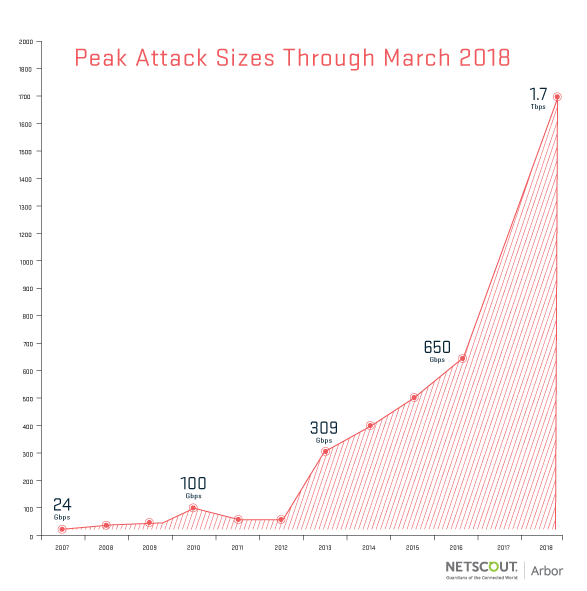
\includegraphics[keepaspectratio,height=.85 \paperheight]{img/DDoS_growth}
	\end{figure}
\end{frame}

\subsection{Reducing Functionality}
\begin{frame}{Reducing Functionality~\cite{Dhanjani:2013:HLSEPHPWLS, Ronen:2018:IGNCZCR, Bhartiya::YSFMK}}
	\note{1m \\
		Disabling things can be very dangerous when more and more of them become connected.

		e.g. blackout entire city with ZLL drive-by attack.
		(image was lightning strike)
		
  	Fridge murder story.
	}
	% We probably can cite something about disabling lights from one of our papers.
	% Other nice things would be fridges or tvs, maybe we can find that?
	% This can dangerous: a smart fridge that thaws meat every night can be deadly!

	% presentation-wise, probably just bullet-points?
	\centering
	\begin{figure}
		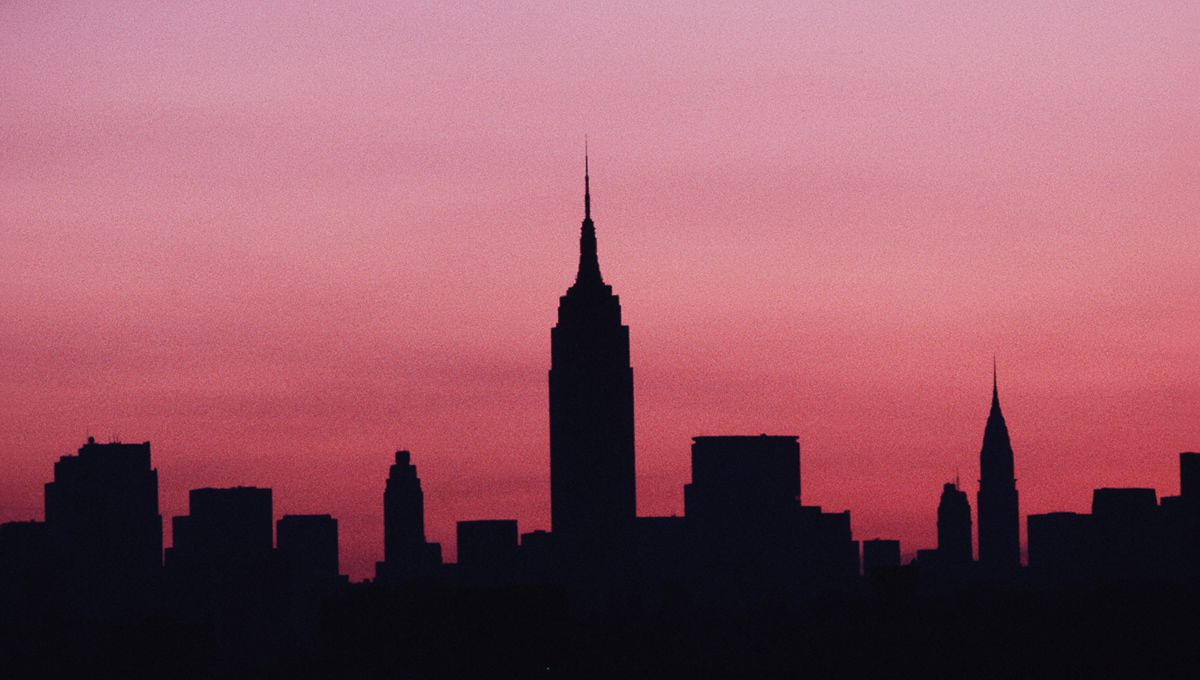
\includegraphics{img/nyc-blackout.jpg}
		\caption{NYC Blackout of 1977 (Allan Tannenbaum/Getty Images)}
	\end{figure}
\end{frame}

\subsection{Misusing Functionality}
\begin{frame}{Misusing Functionality}
	\note{30s \\
		This is probably more annoying than dangerous.

	}
	\begin{block}{Create Discomfort}
		\begin{itemize}
			\item Heat in summer, AC in winter
			\item Flash bedroom lights at night
			\item Turn on AC in bathroom in the morning
		\end{itemize}
	\end{block}
	\begin{block}{Generally be Annoying}
		\begin{itemize}
			\item Turn on lights
			\item Open Faucets
			\item Run Washing Machine
		\end{itemize}
		\pause{}
		\dots~when the owners leave for vacation.
	\end{block}
\end{frame}

\subsection{Extending Functionality}
	% TODO The interesting things. I like the examples from the paper:
	% Start a fire with AC, unlock front door with roomba (vacuum cleaner robot)
  % It seems like no other author has worked on this...
	% Any idea of how to visualize that?
\begin{frame}{Extending Functionality~\cite{Ronen:2016:EFAIDCSL,Guri:2017:xCDEANvRL}}
	\note{30s \\
		\begin{itemize}
			\item Most interesting
			\item Almost no reseach (Ronen, Guri (Router LEDs))
		\end{itemize}
	}
    \only<+>{
        \begin{block}{Possible Extending Functionality Attacks}
            \begin{itemize}
                \item Open front door with smart household robots
                \item Start a fire with an AC
            \end{itemize}
        \end{block} 
        \vspace{0.5cm}
        \centering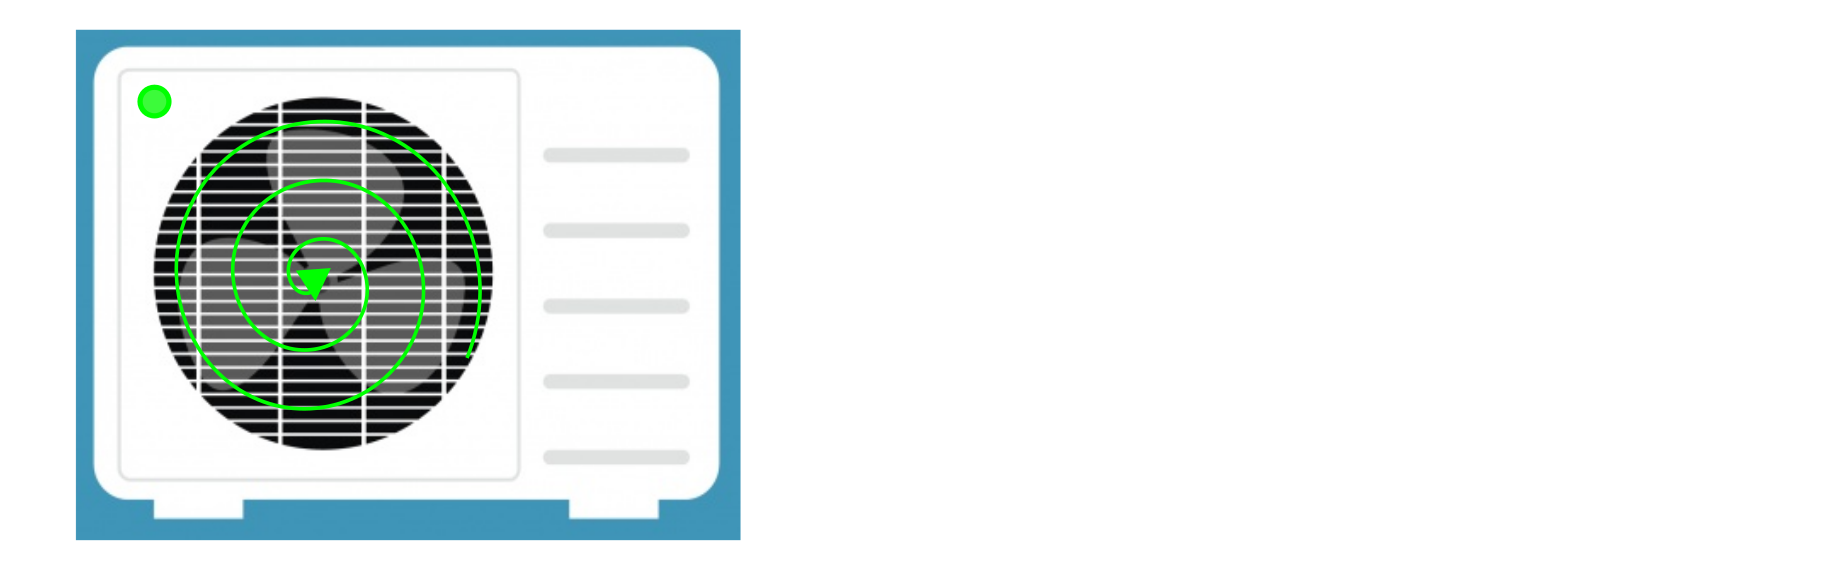
\includegraphics{img/AC-attack_1.png}
    }
    \only<+>{\centering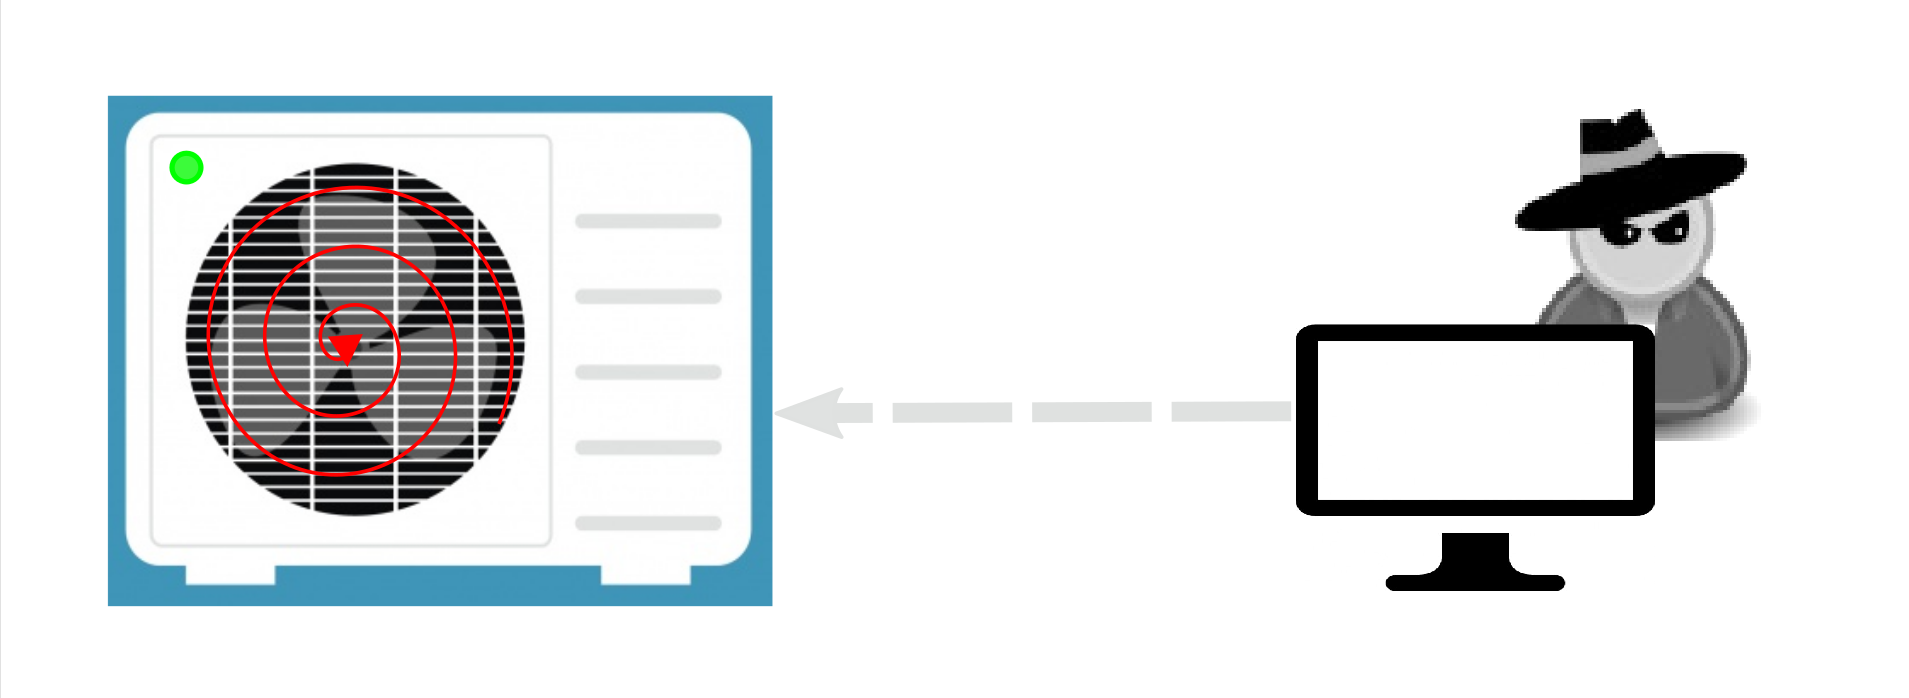
\includegraphics{img/AC-attack_2.png}}
    \only<+>{\centering
\includegraphics{img/AC-attack_3.png}}  
\end{frame}

\begin{frame}{Extending Functionality --- The Case of Smart Lights}
	\note{30s \\
		Interesting because light is often the only part of the EM-spectrum that is allowed to leave air-gapped systems.
	}
    \only<+>{\centering
\includegraphics{img/DatacenterIoT_1.png}}
    \only<+>{\centering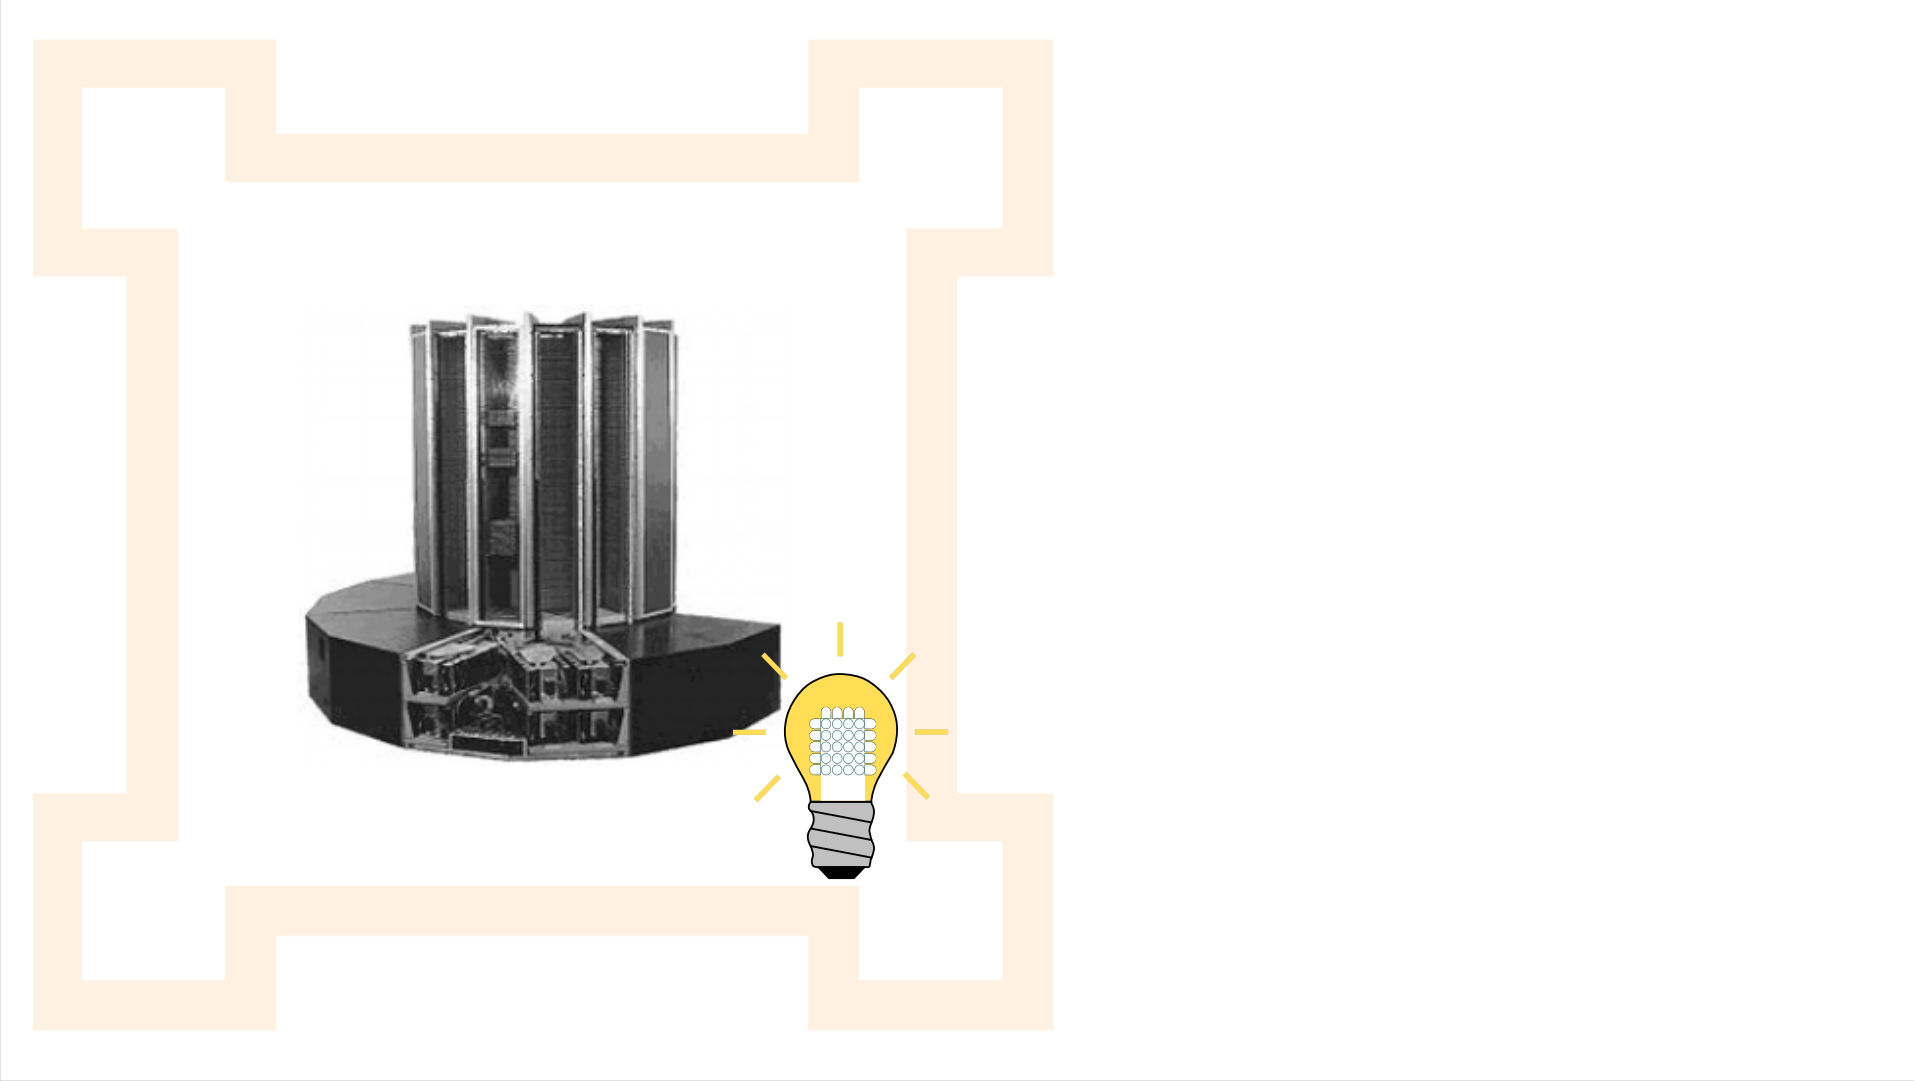
\includegraphics{img/DatacenterIoT_2.png}}
    \only<+>{\centering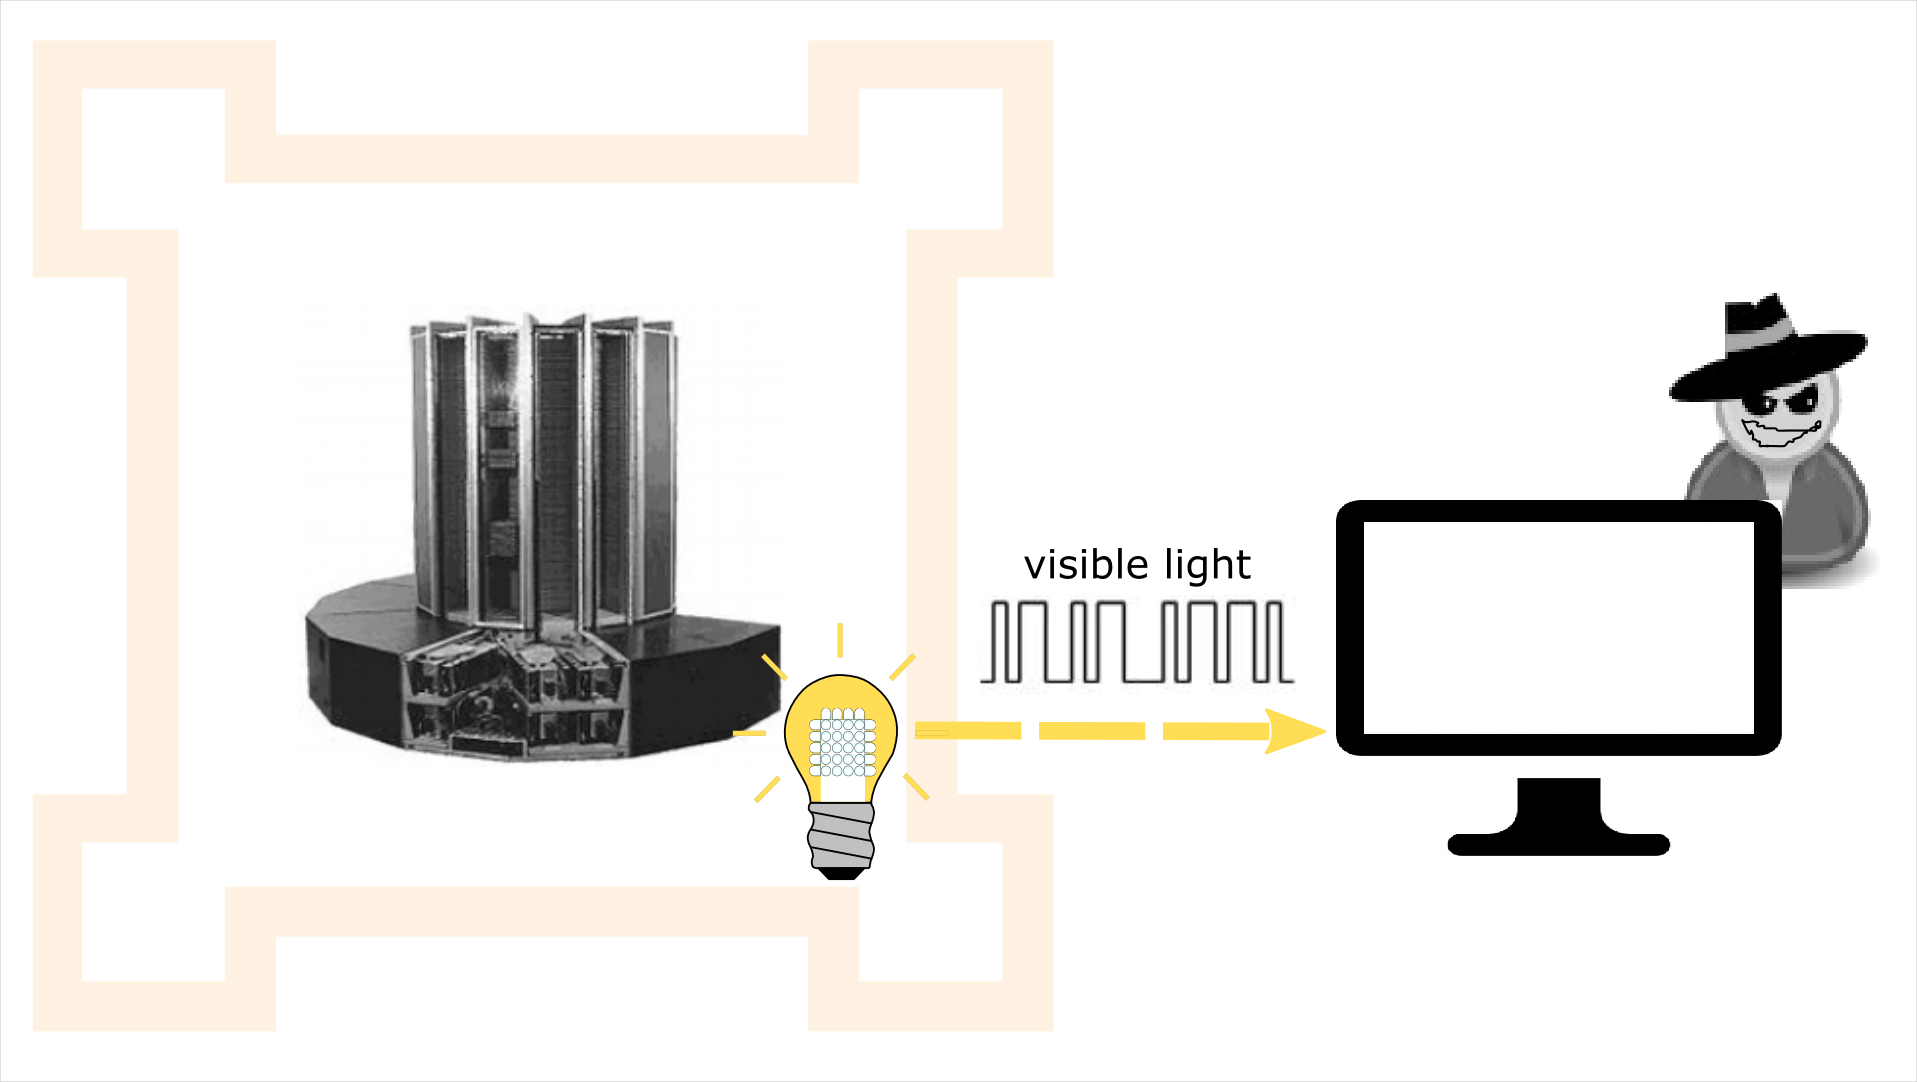
\includegraphics{img/DatacenterIoT_3.png}}
    \only<+>{\centering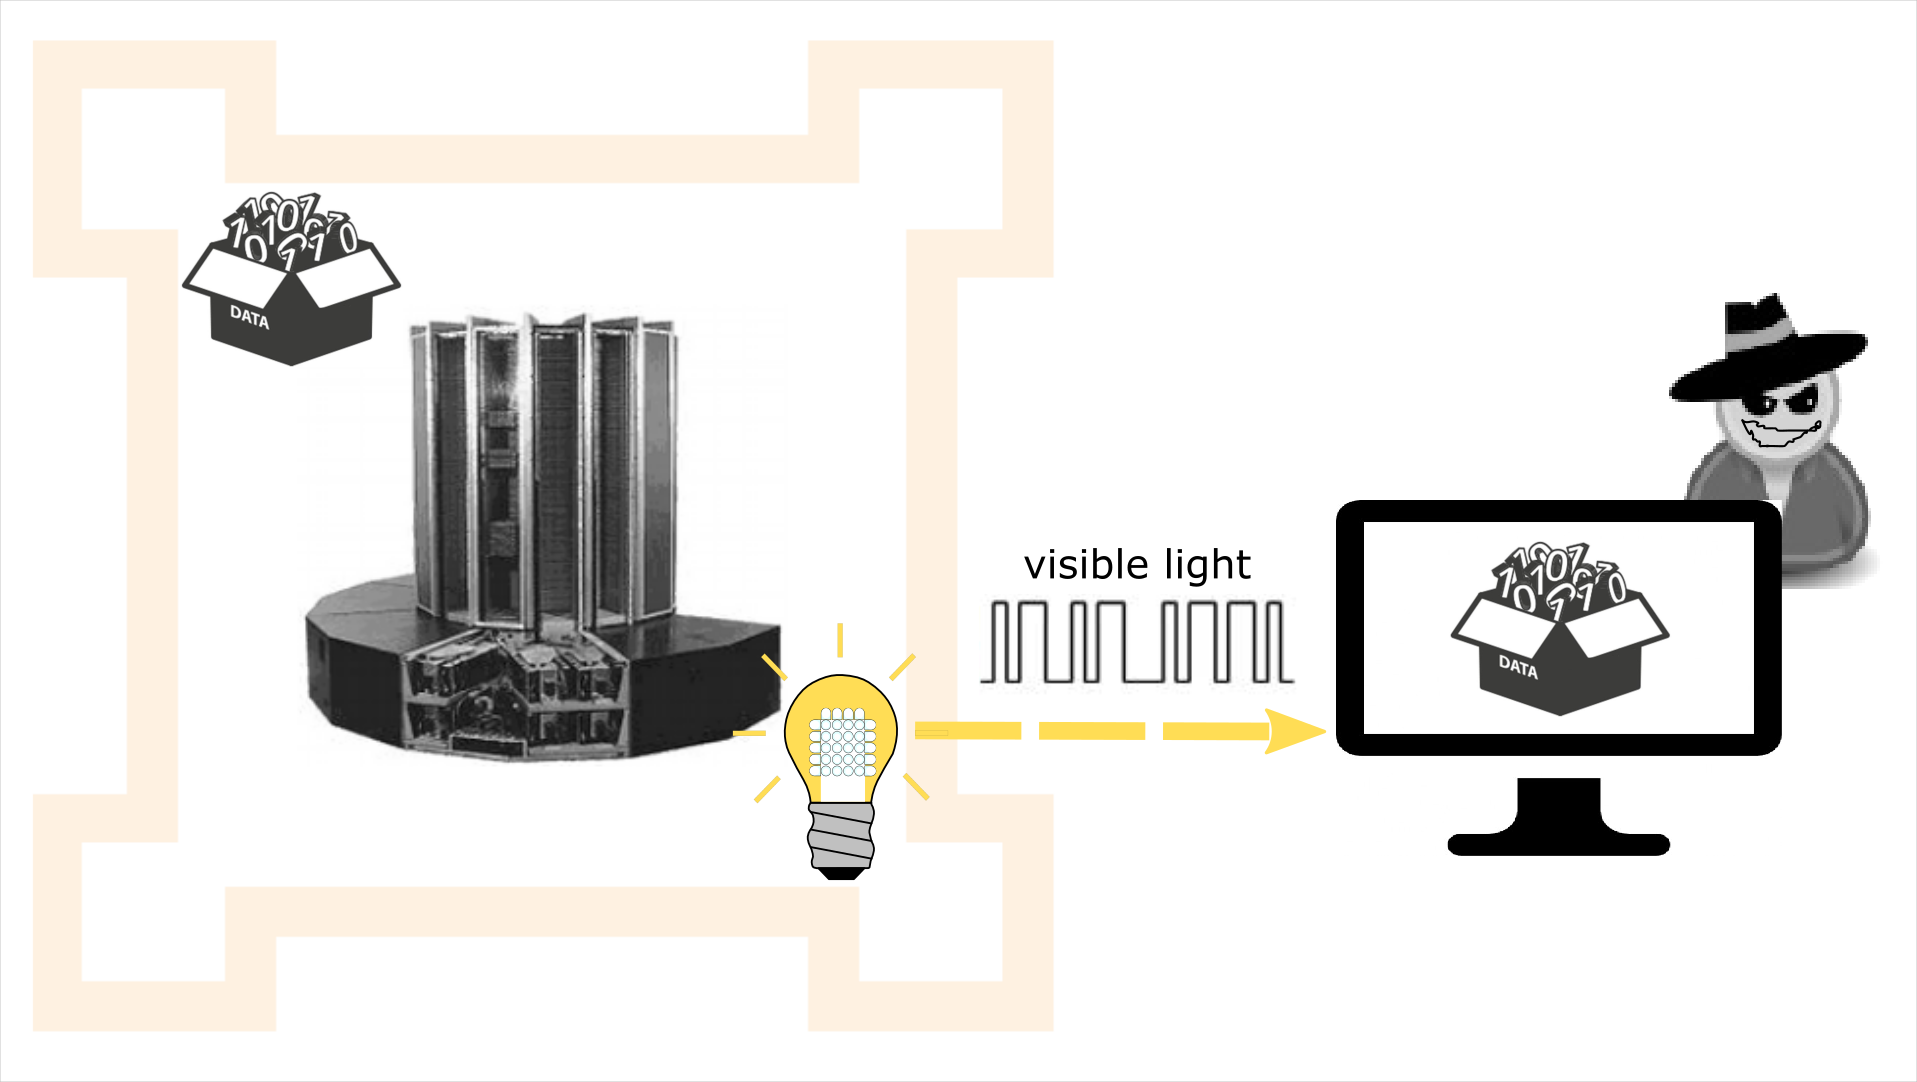
\includegraphics{img/DatacenterIoT_4.png}}
\end{frame}

\title{E. Ronen and A. Shamir Paper}
\subtitle{Extended Functionality Attacks on IoT Devices: The Case of Smart Lights}
\section{E. Ronen and A. Shamir Paper}

\subsection{Covert Channel}%
\label{sub:covert_channel}

\subsubsection{Requirements for Covert Channel}%
\label{sub:requirements_for_covert_channel}
\begin{frame}{Requirements for Covert Channel}
	\begin{block}{Correctness}
		Switch between 2 brightnesses that can be robustly distinguished by a sensor.
	\end{block}
	\begin{block}{Covertness}
		Use brightnesses so similar or switch so fast that a human cannot distinguish them.
	\end{block}
	
	%TODO: show gif led-flickering (taken from PubNub - Building the Raspberry Pi Smart House: Controlling Lights with PWM)

\end{frame}
% with info about human eyes

\subsubsection{How (smart) LEDs Work}%
\label{sub:how_smart_leds_work}
% TODO
% with info about controller, ZLL, and PWM duty cycle for brightness
% Probably want to add a duty cycle/brightness diagram or something.
\begin{frame}{How (smart) LEDs Work}
    \only<1> {
        \begin{block}{RF Receiver (and transmitter)}
            \begin{itemize}
                \item For communication with controller
								\item Communicate with ZigBee Light Link (ZLL)~\cite{Ronen:2018:IGNCZCR}
            \end{itemize}
        \end{block}
    }
    \only<2> {
        % TODO add pic ZLL communication
         \begin{figure}
            \centering
            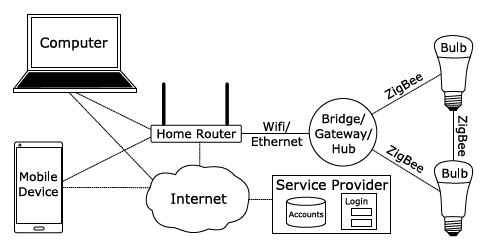
\includegraphics[height=5cm,keepaspectratio]{img/ZLL.JPG}
            \caption{\small{System architecture of a ZLL-based connected lighting system with two bulbs} \footnote{\tiny{Morgner et al. All Your Bulbs Are Belong to Us: Investigating the Current State of Security in Connected Lighting Systems}}}
         \end{figure}
    }
    \only<3> {
        \begin{block}{Processing Unit}
            \begin{itemize}
                \item For processing commands received from controller
								\item LEDs are controlled using pulse width modulation (PWM) signals~\cite{Yu:2014:BCDRCVLOS,Elgala:2007:OVLWCBoWL}
            \end{itemize}
        \end{block}
        
        \begin{block}{Drivers and LEDs}
            \begin{itemize}
                \item Driver controls LED on and off states
                \item Determine brightness level of bulb
            \end{itemize}
        \end{block}
    }
    \only<4> {
         % TODO add illustration brightness control (PWM duty cycle method and according brightness change)
         
        \begin{figure}
            \centering
            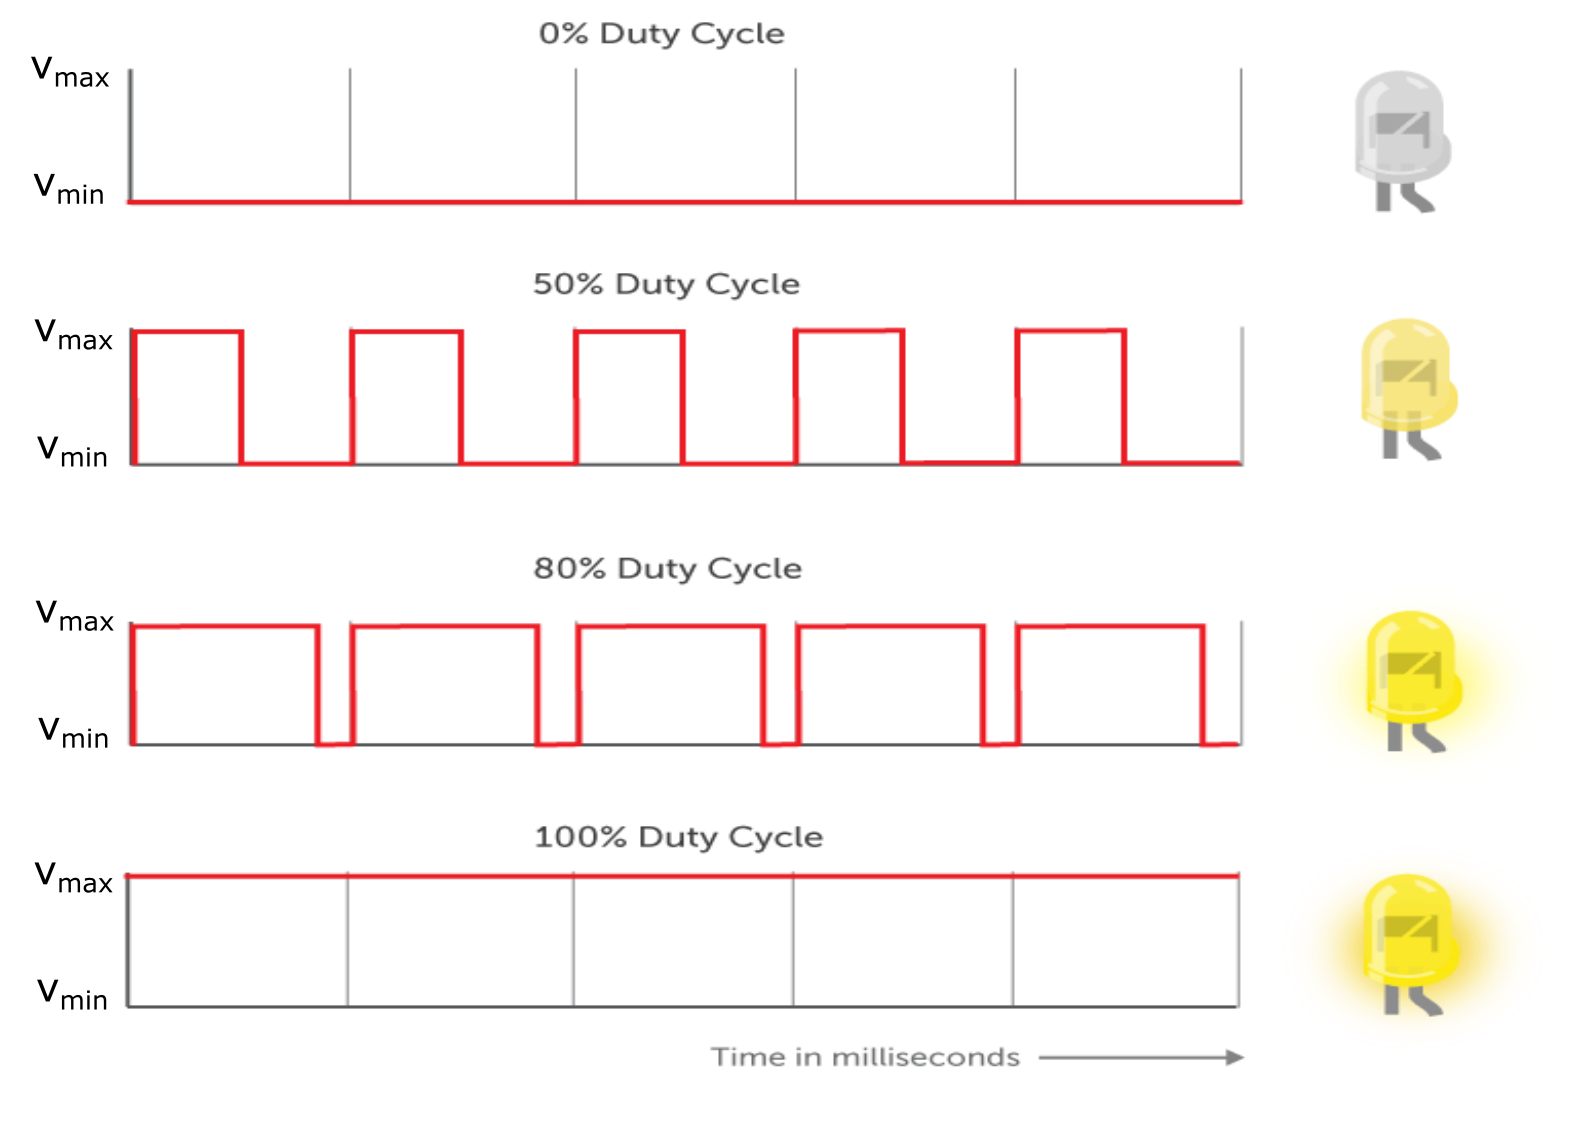
\includegraphics[height=5.5cm,keepaspectratio]{img/pwm-duty-cycle.png}
            \caption{\small{Brightness control on LEDs} \footnote{\tiny{PubNub - Building the Raspberry Pi Smart House: Controlling Lights with PWM}}}
        \end{figure}
    }
\end{frame}

% TODO: the following sections cover attacking limitless led only, should we add philips too? - if yes please just tell me how they accessed the controller to actually send the api commands which further allowed the flickering - since I don't understand although I read the paper several times now...

\subsubsection{Encoding: Crafting of PWM Signals}%
\label{sub:encoding_crafting_of_pwm_signals}
% TODO
% - Talk about attacking/using the controller
% - Talk about how to make sufficiently fast changes
% - Diagram of the resulting signals?
\begin{frame}{Encoding: Access Controller}
% description based on LimitlessLED
    \only<1> {
        \centering
        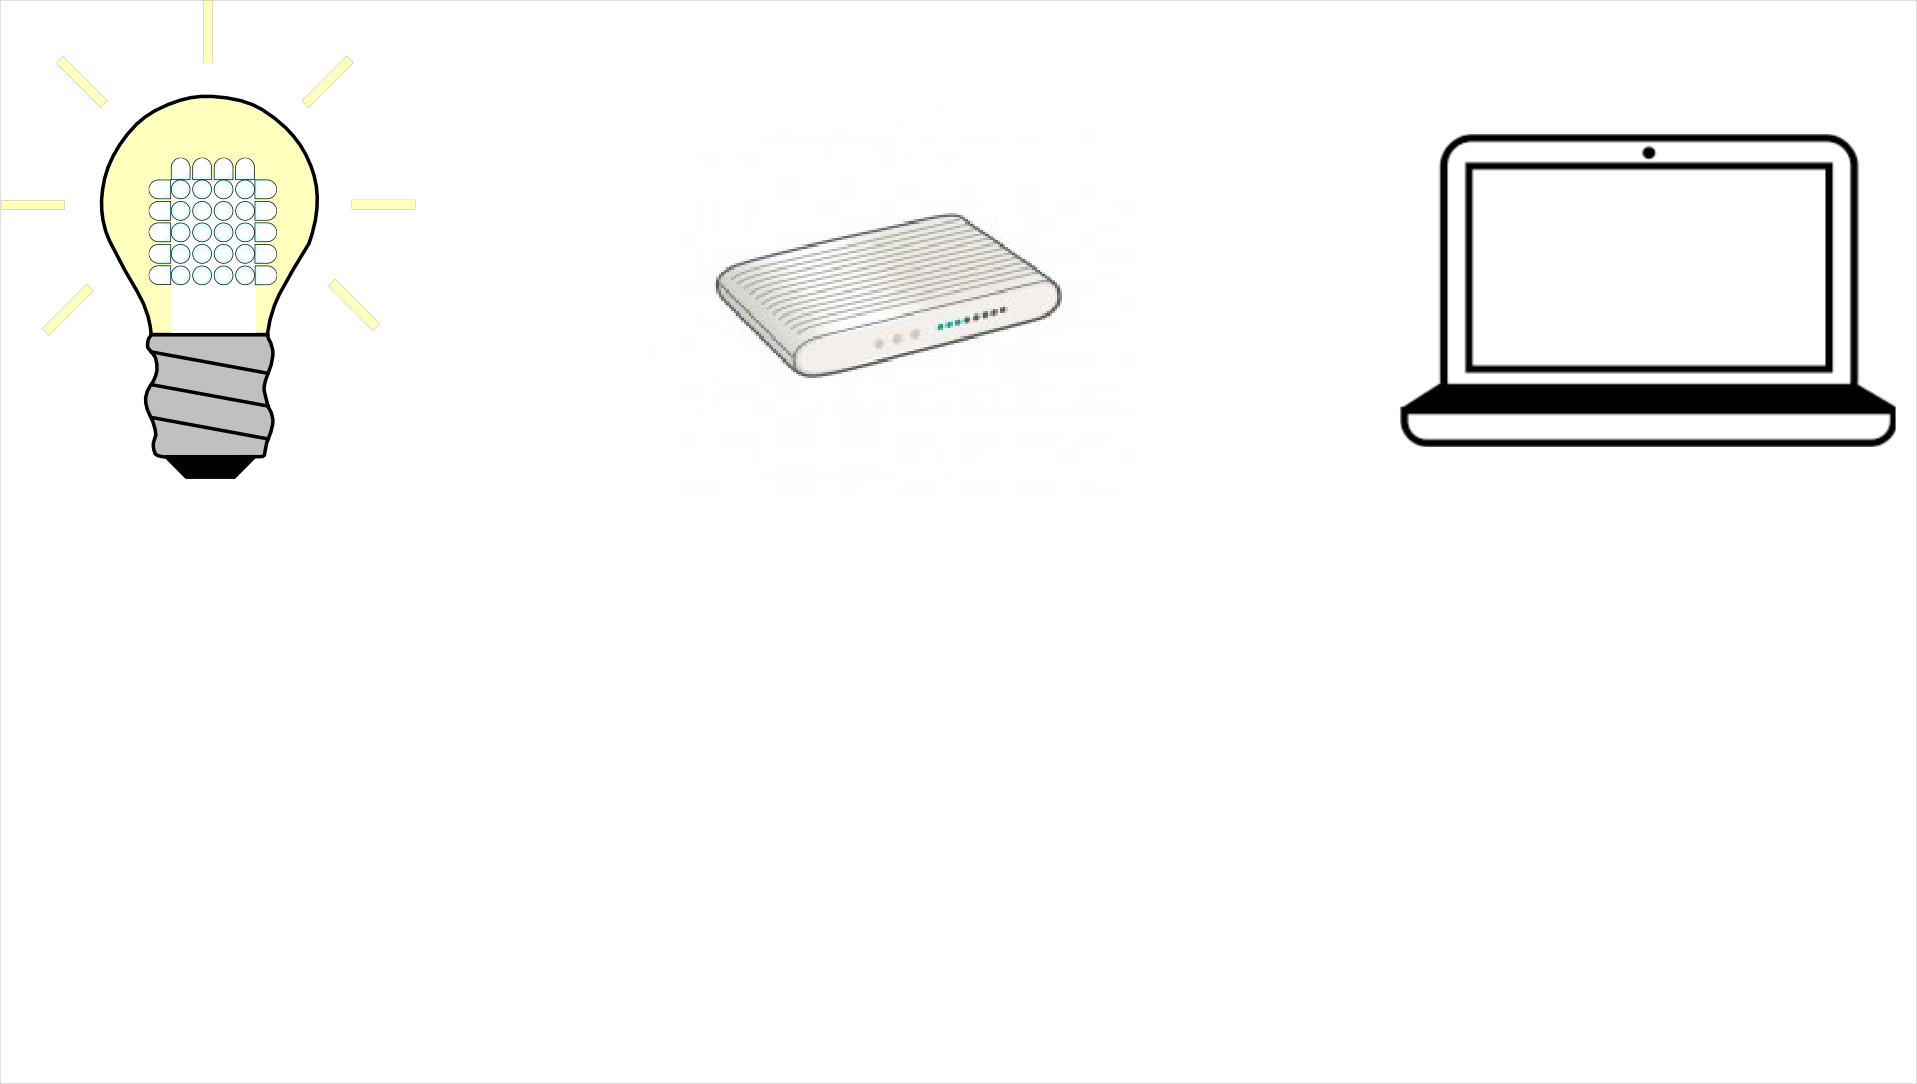
\includegraphics{img/AttackController_1.png}
    }
    \only<2> {
        \centering
        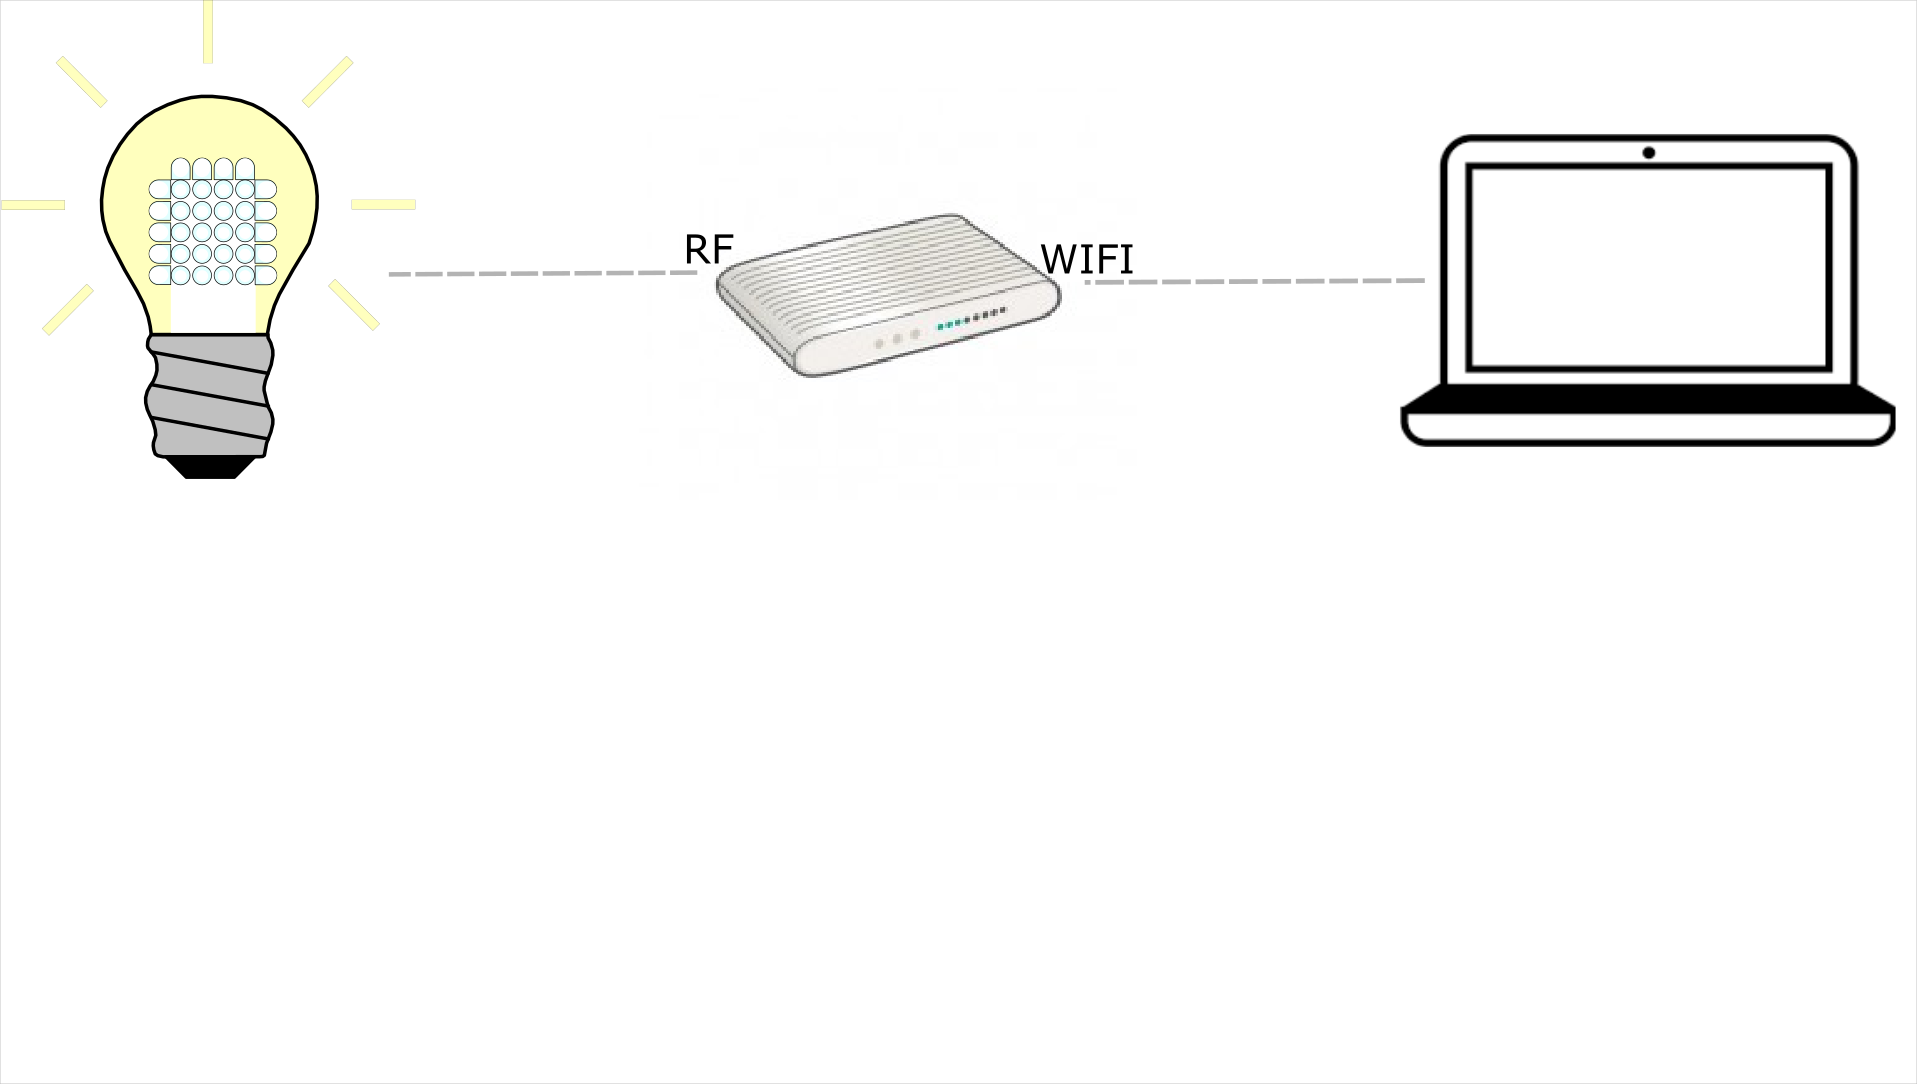
\includegraphics{img/AttackController_2.png}
    }
    \only<3> {
        \centering
        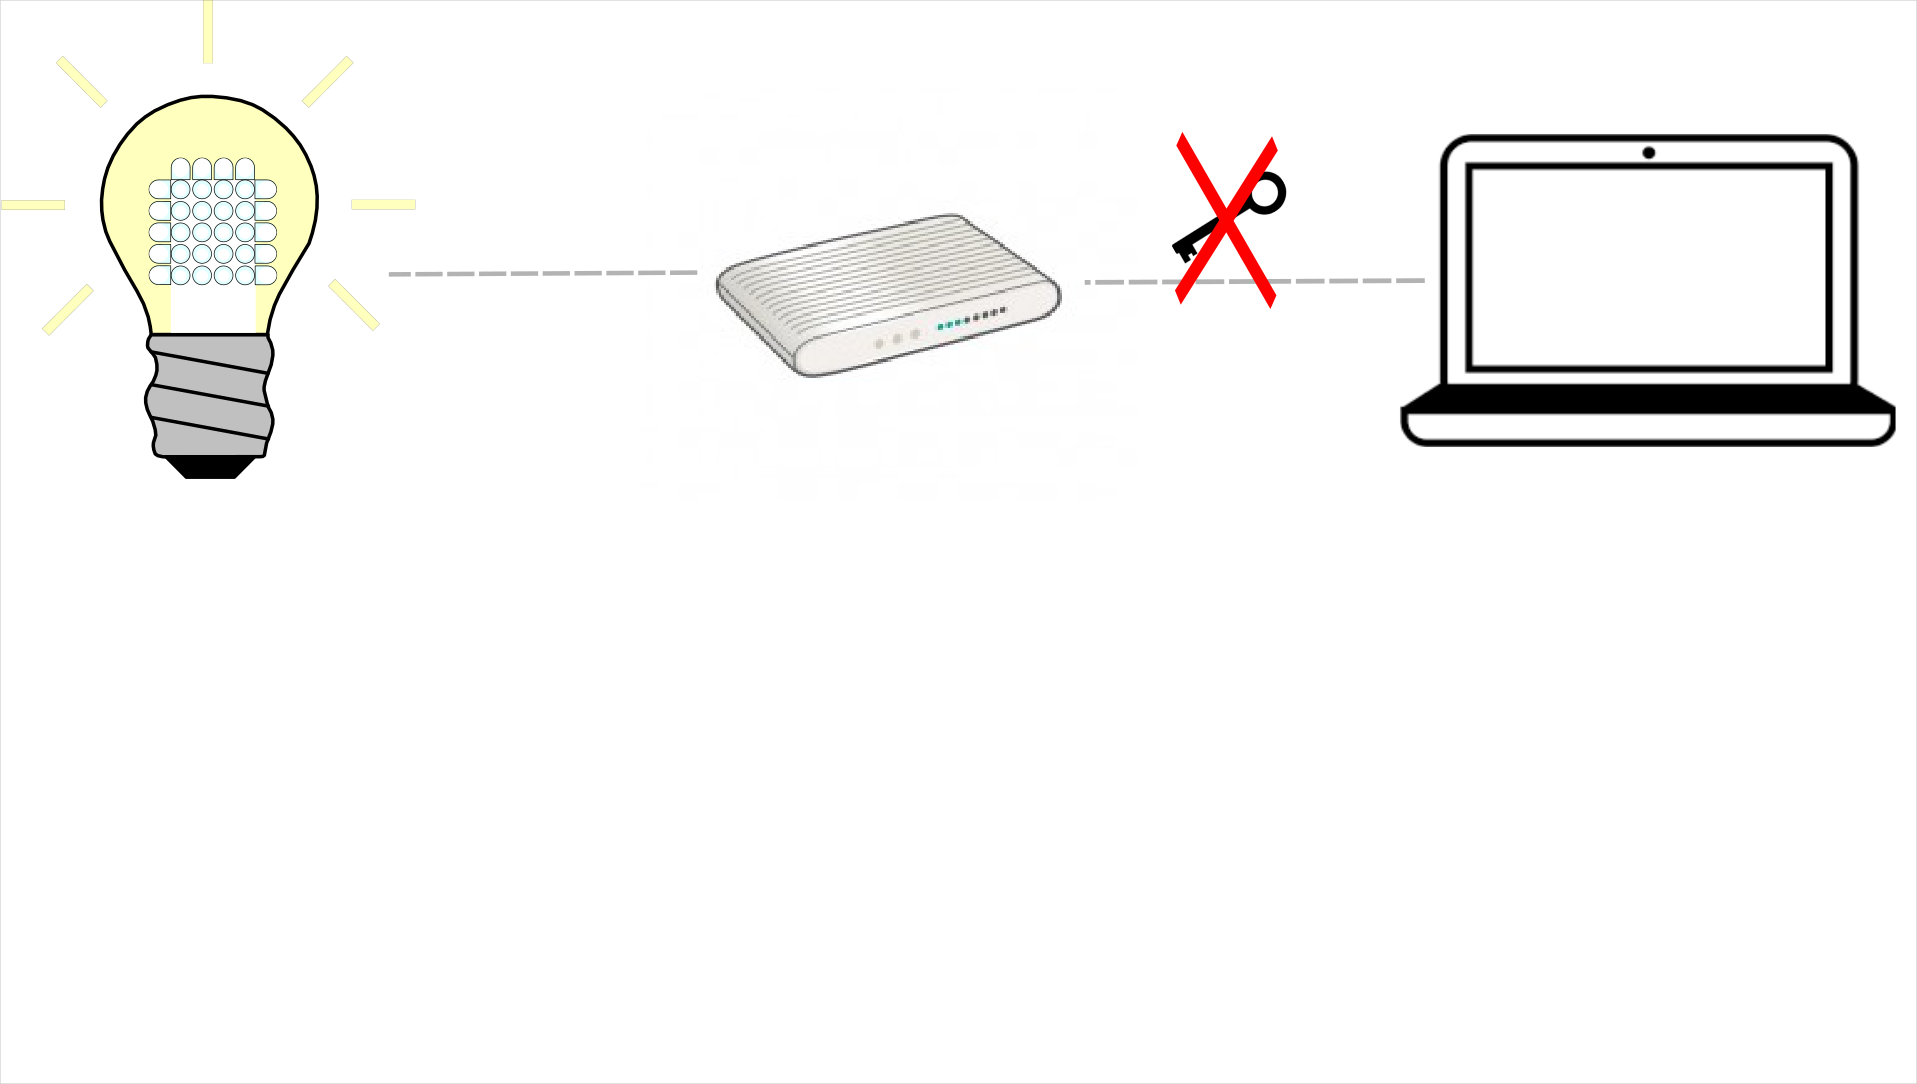
\includegraphics{img/AttackController_3.png}
    }
    \only<4> {
        \centering
        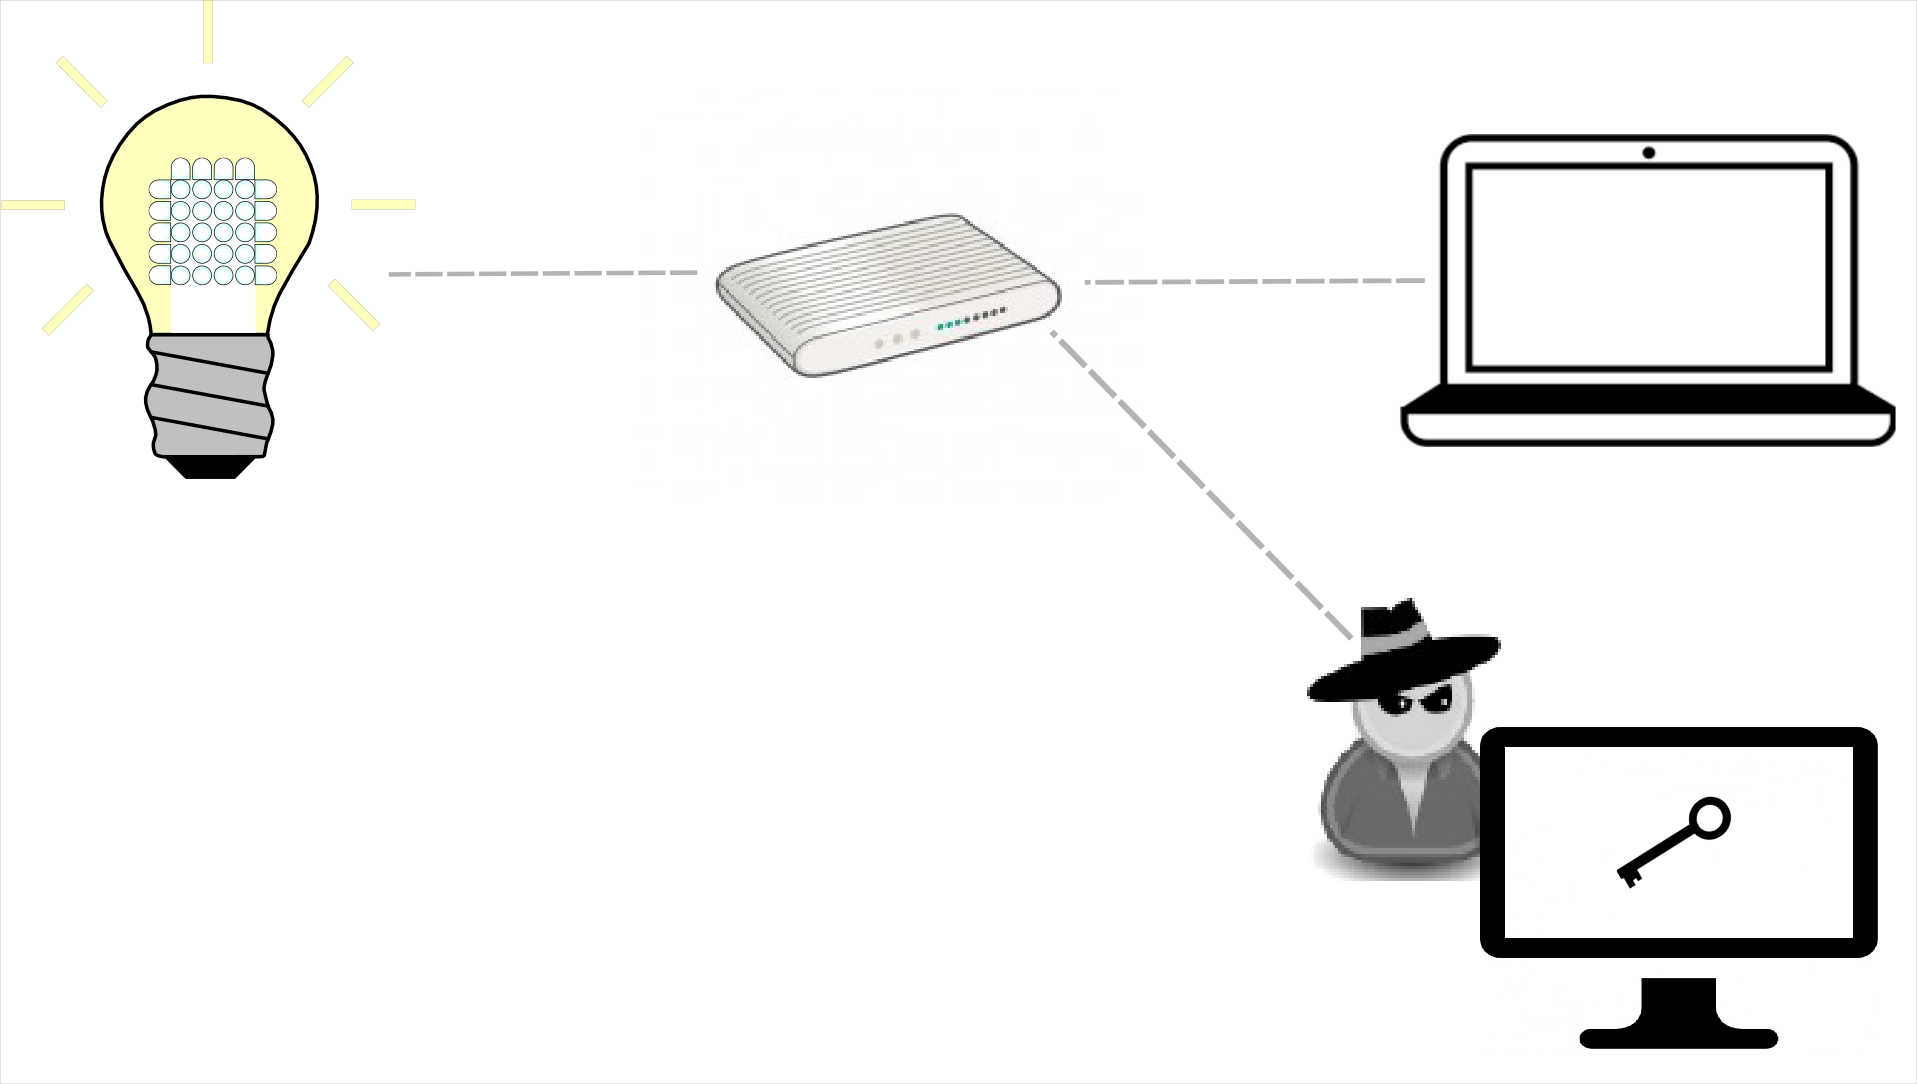
\includegraphics{img/AttackController_4.png}
    }
    \only<5> {
        \centering
        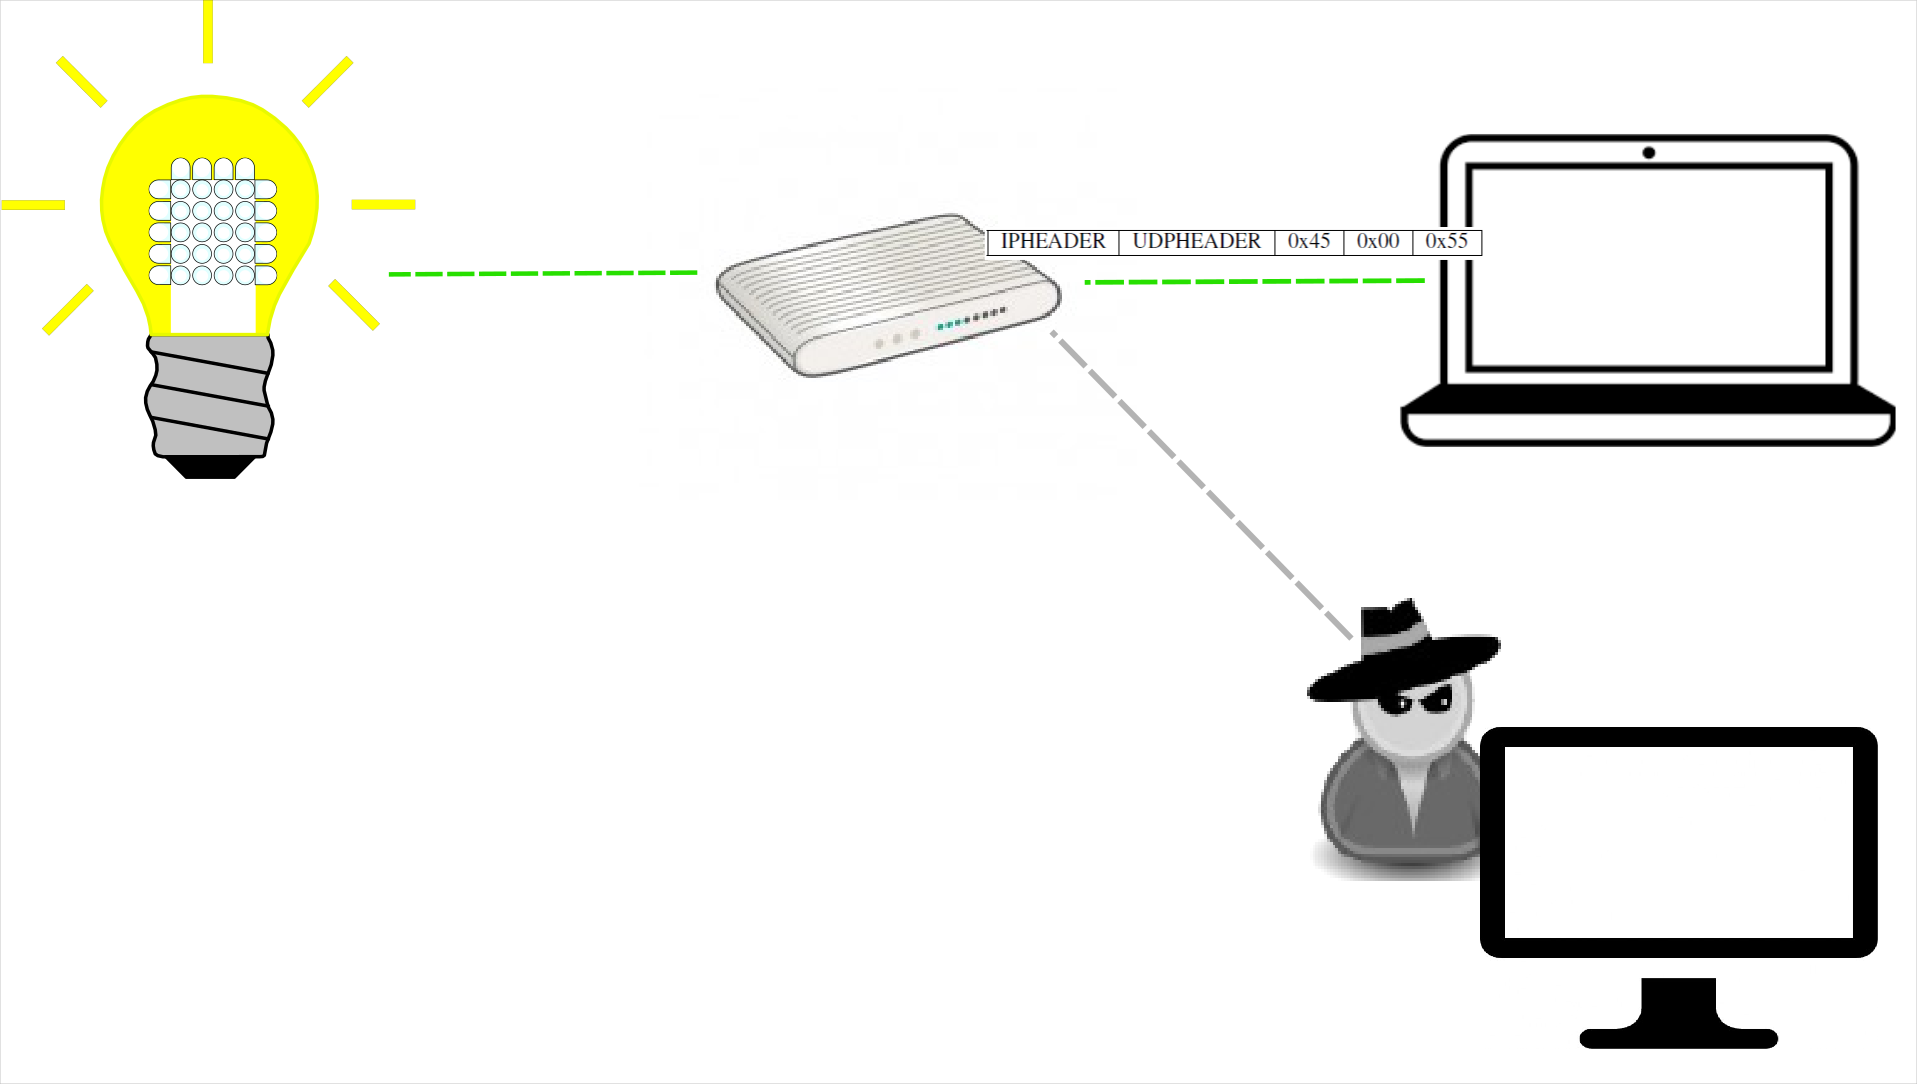
\includegraphics{img/AttackController_5.png}
    }
    \only<6> {
        \centering
        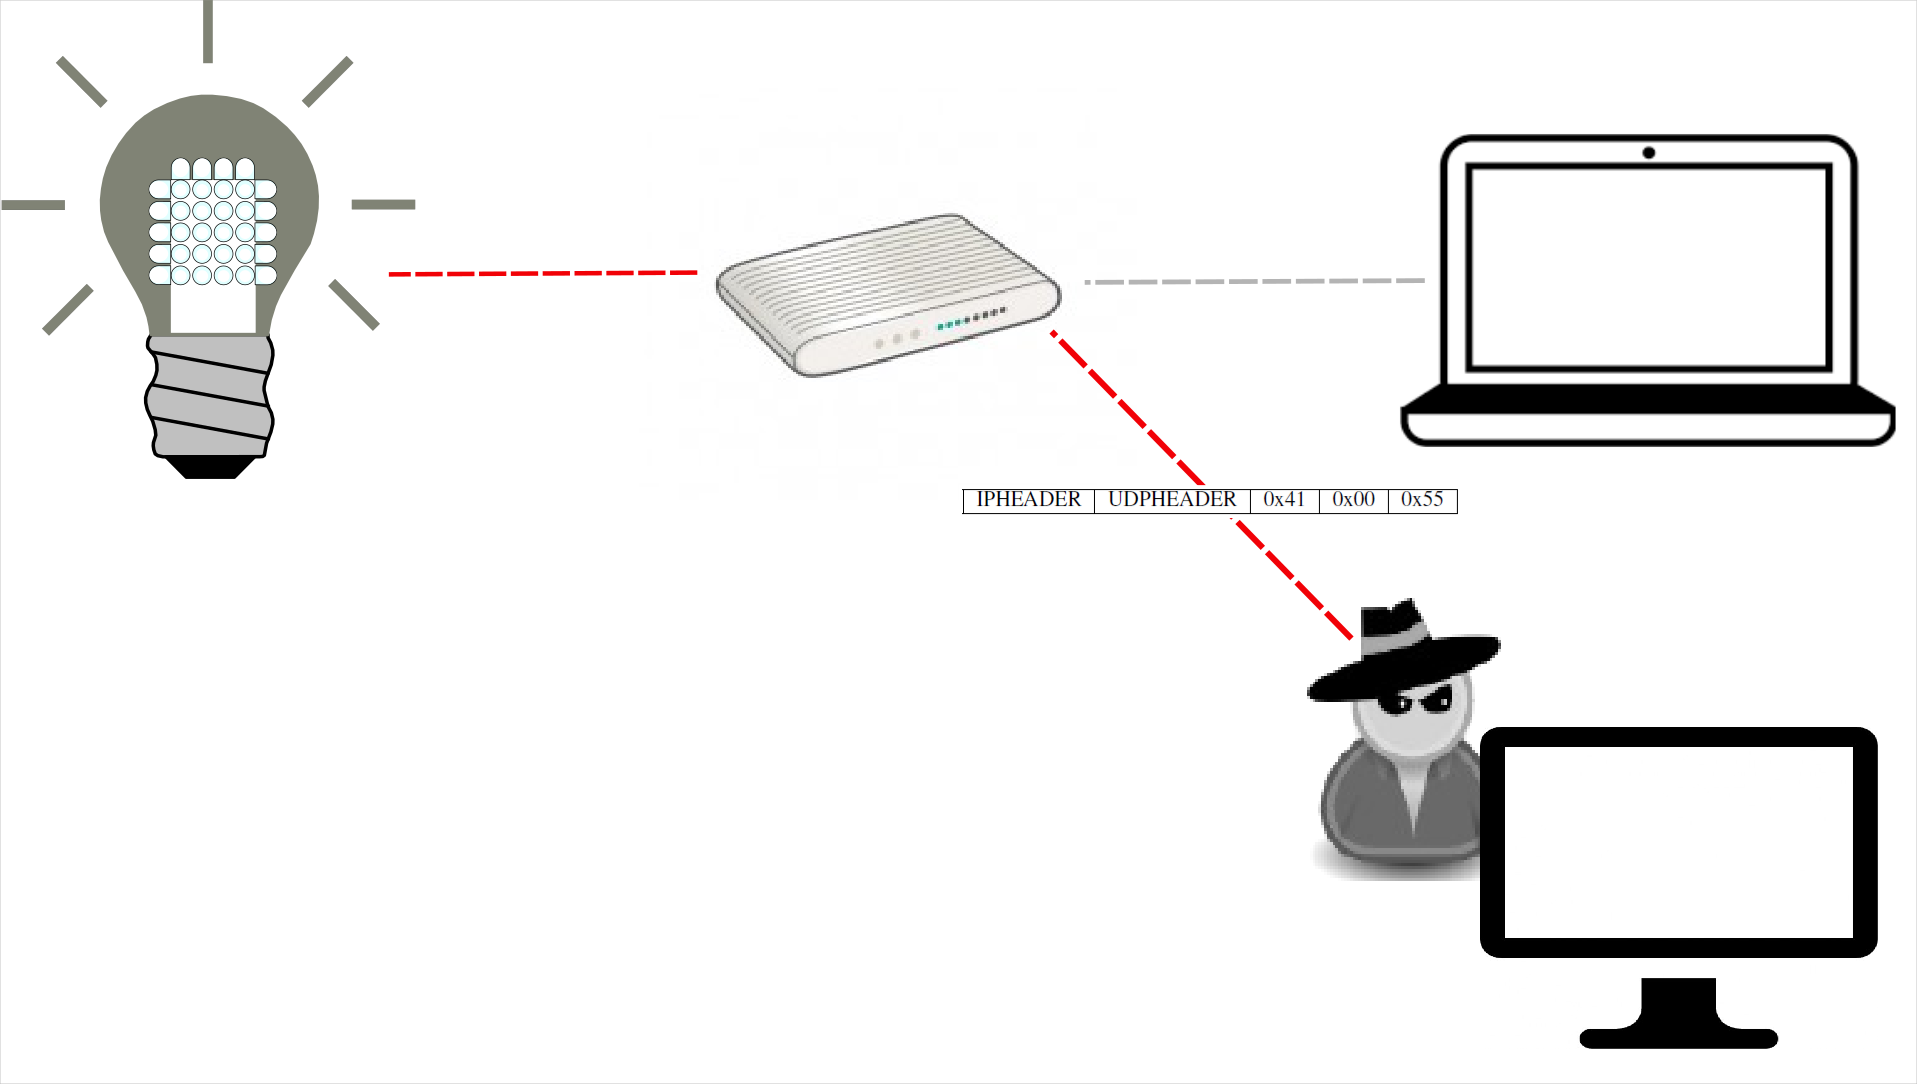
\includegraphics{img/AttackController_6.png}
    }
\end{frame}

\begin{frame}{Encoding: Crafting of PWM Signals}
    % TODO: describe, + diagram of resulting signal
    % Philips: send undocumented API command to flicker at high rate
    
    % 1: Limitless: repeatedly send low commands followed by high commands to flicker at high rate
    \begin{figure}
        \centering
        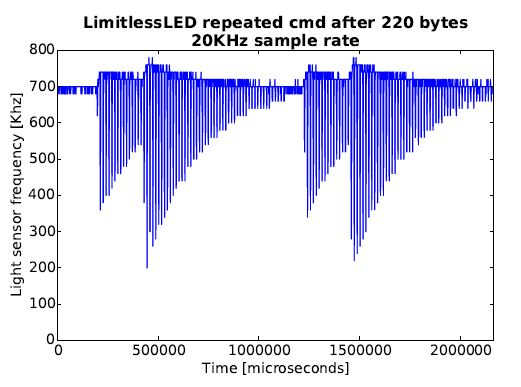
\includegraphics[height=5.5cm,keepaspectratio]{img/fast-flickering_limitlessLED.JPG}
        \caption{\small{Smooth control of PWM duty cycle \footnote{\tiny{Ronen and Shamir. Extended Functionality Attacks on IoT Devices: The Case of Smart Lights}}}}
    \end{figure}
    
     
\end{frame}

% Need to think about whether we want to cover LimitlessLED/LUX old/LUX new or only one of them!
% --> it's hard.. I'd say LimitlessLED since PWM signal analysis can be done more easily (according to paper), and there are known setup vulnerabilities (if we use the same version), BUT we'd then have less intensity values which will make it harder creating a real covert channel - BUT 3 top brightness levels of LimitlessLED are the same, so maybe those levels can be used in order to keep channel covert - so I'm not sure about that thought 
\subsubsection{Decoding: Light Sensor Signal Analysis}%
\label{sub:decoding_light_sensor_signal_analysis}
% TODO -> graphical illustration on slides, according description done verbally
% - Describe receiving hardware setup
% - Describe how the signal can be processed to get a bit stream
\begin{frame}{Decoding: Light Sensor Signal Analysis}
    \only<1> {
        \centering
        
\includegraphics{img/Decoding_1.png}
    }
    \only<2> {
        \centering
        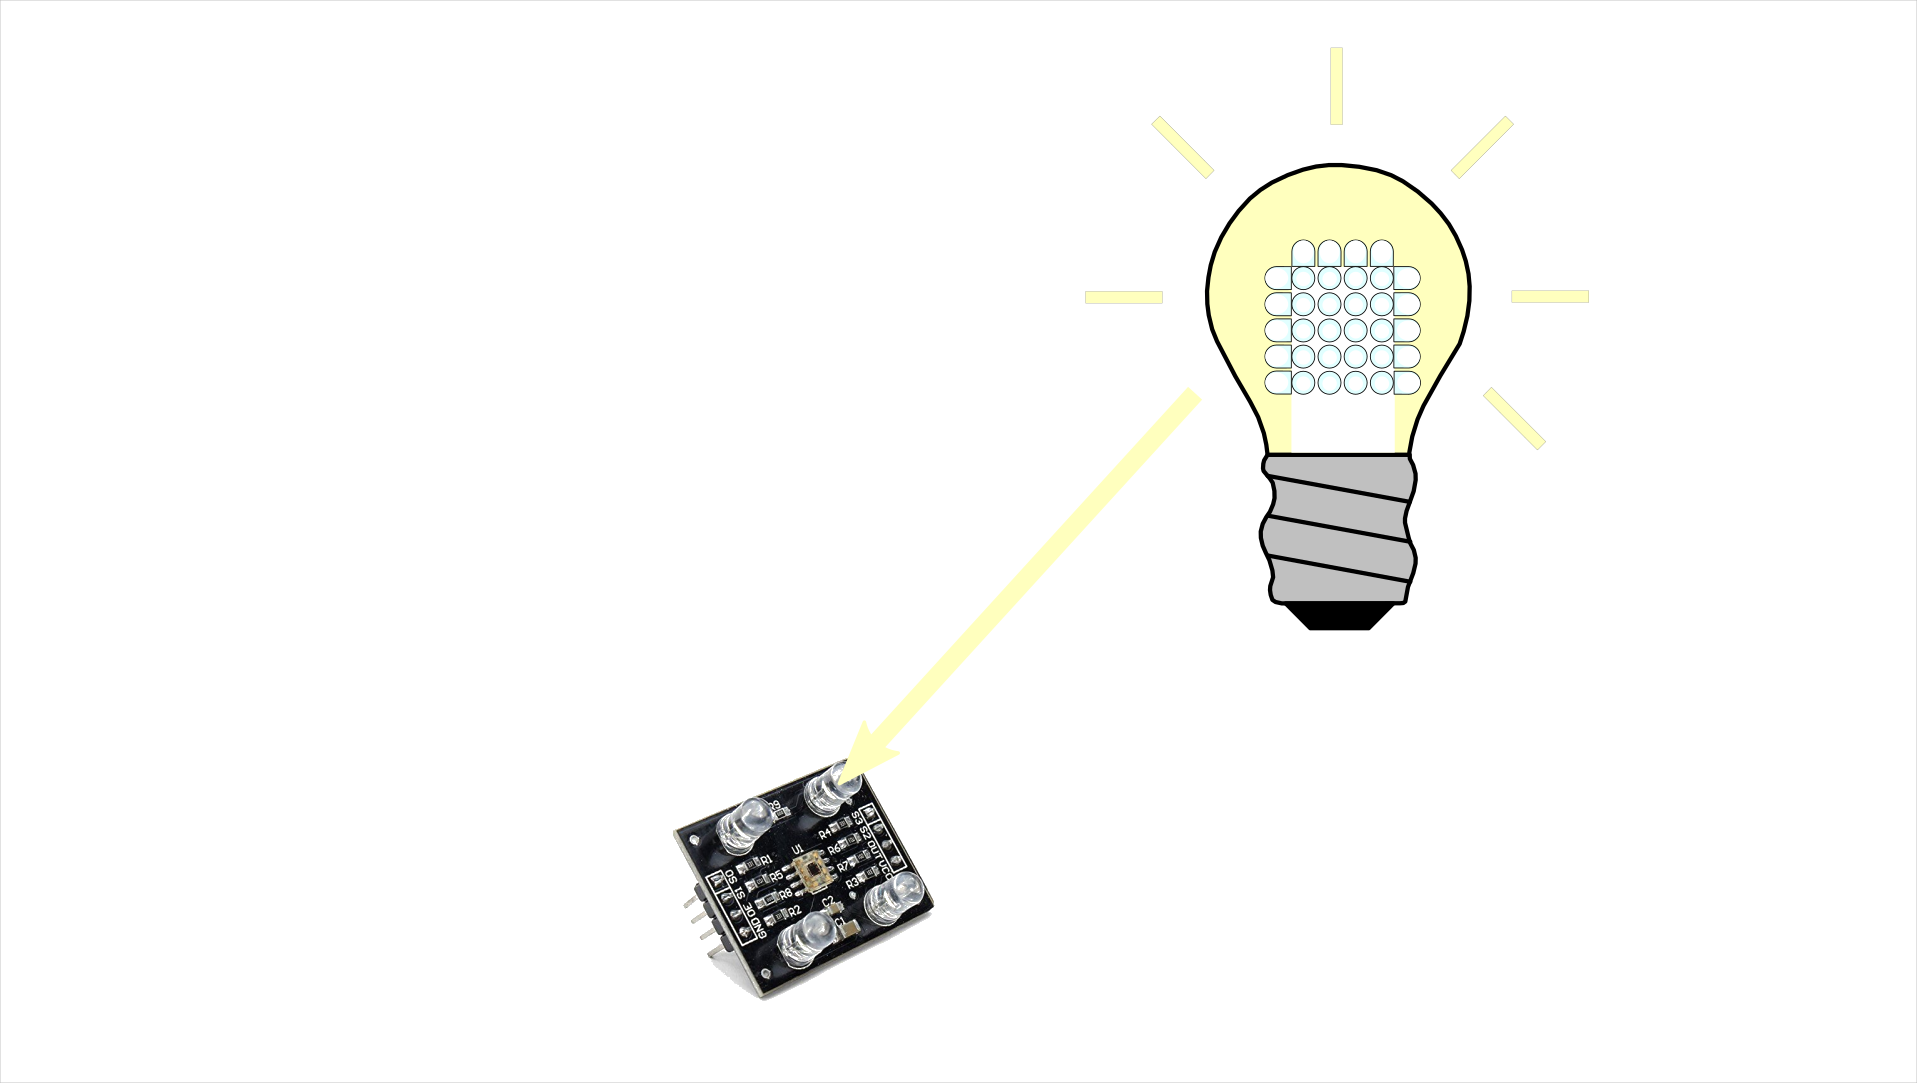
\includegraphics{img/Decoding_2.png}
    }
    \only<3> {
        \centering
        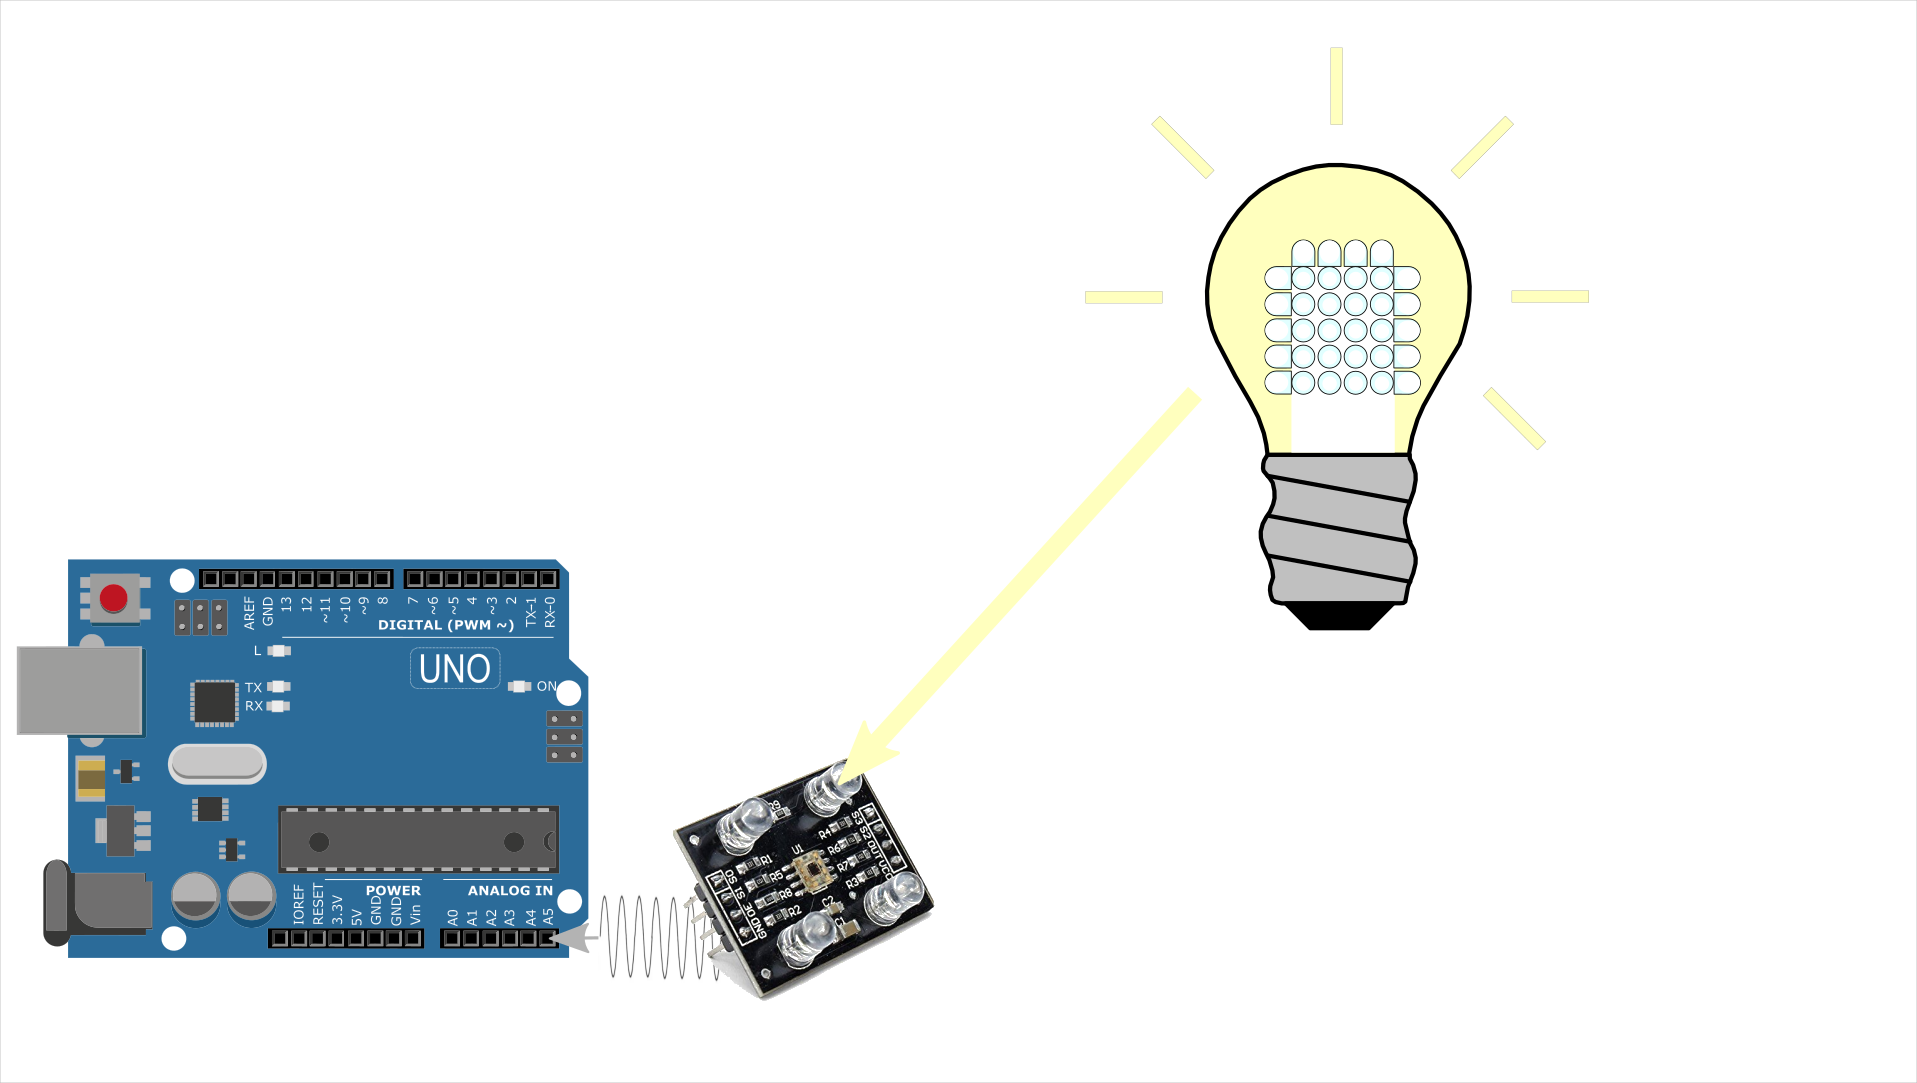
\includegraphics{img/Decoding_3.png}
    }
    \only<4> {
        \centering
        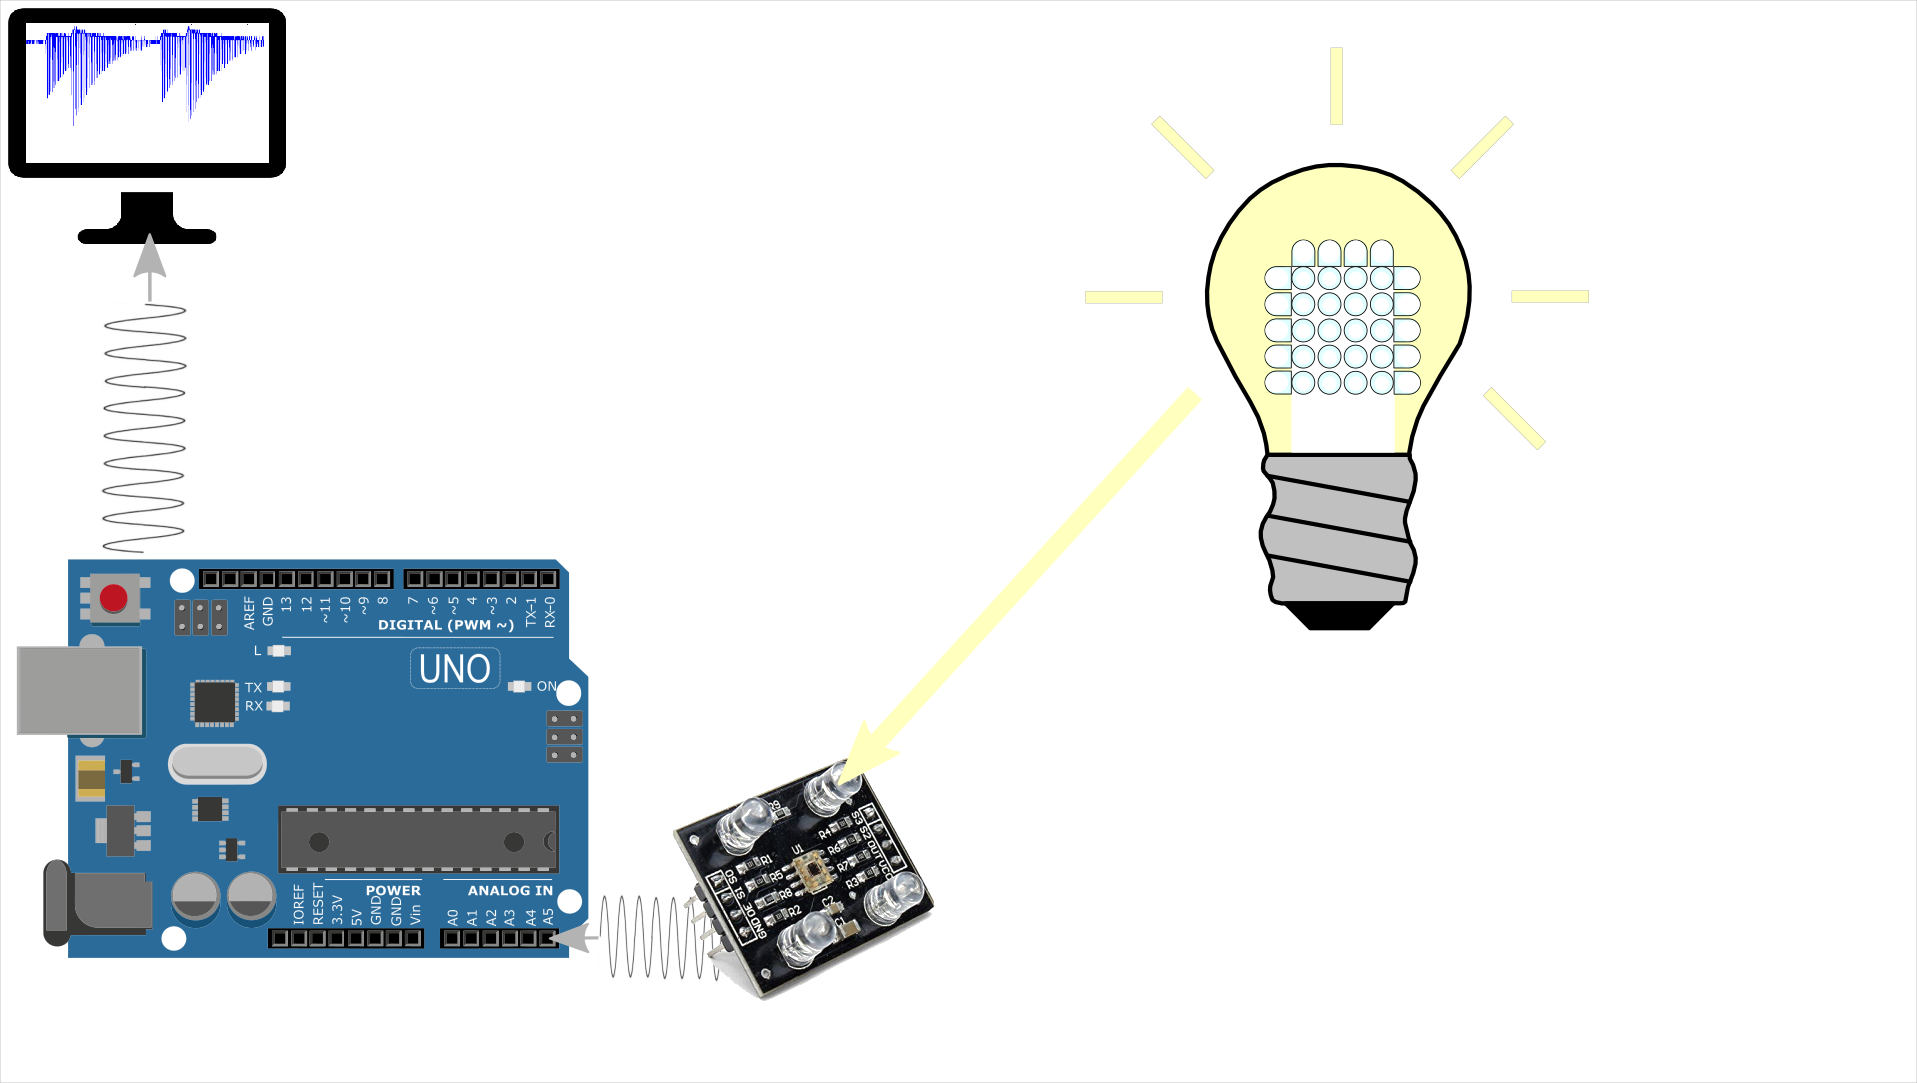
\includegraphics{img/Decoding_4.png}
    }
    \only<5> {
        \centering
        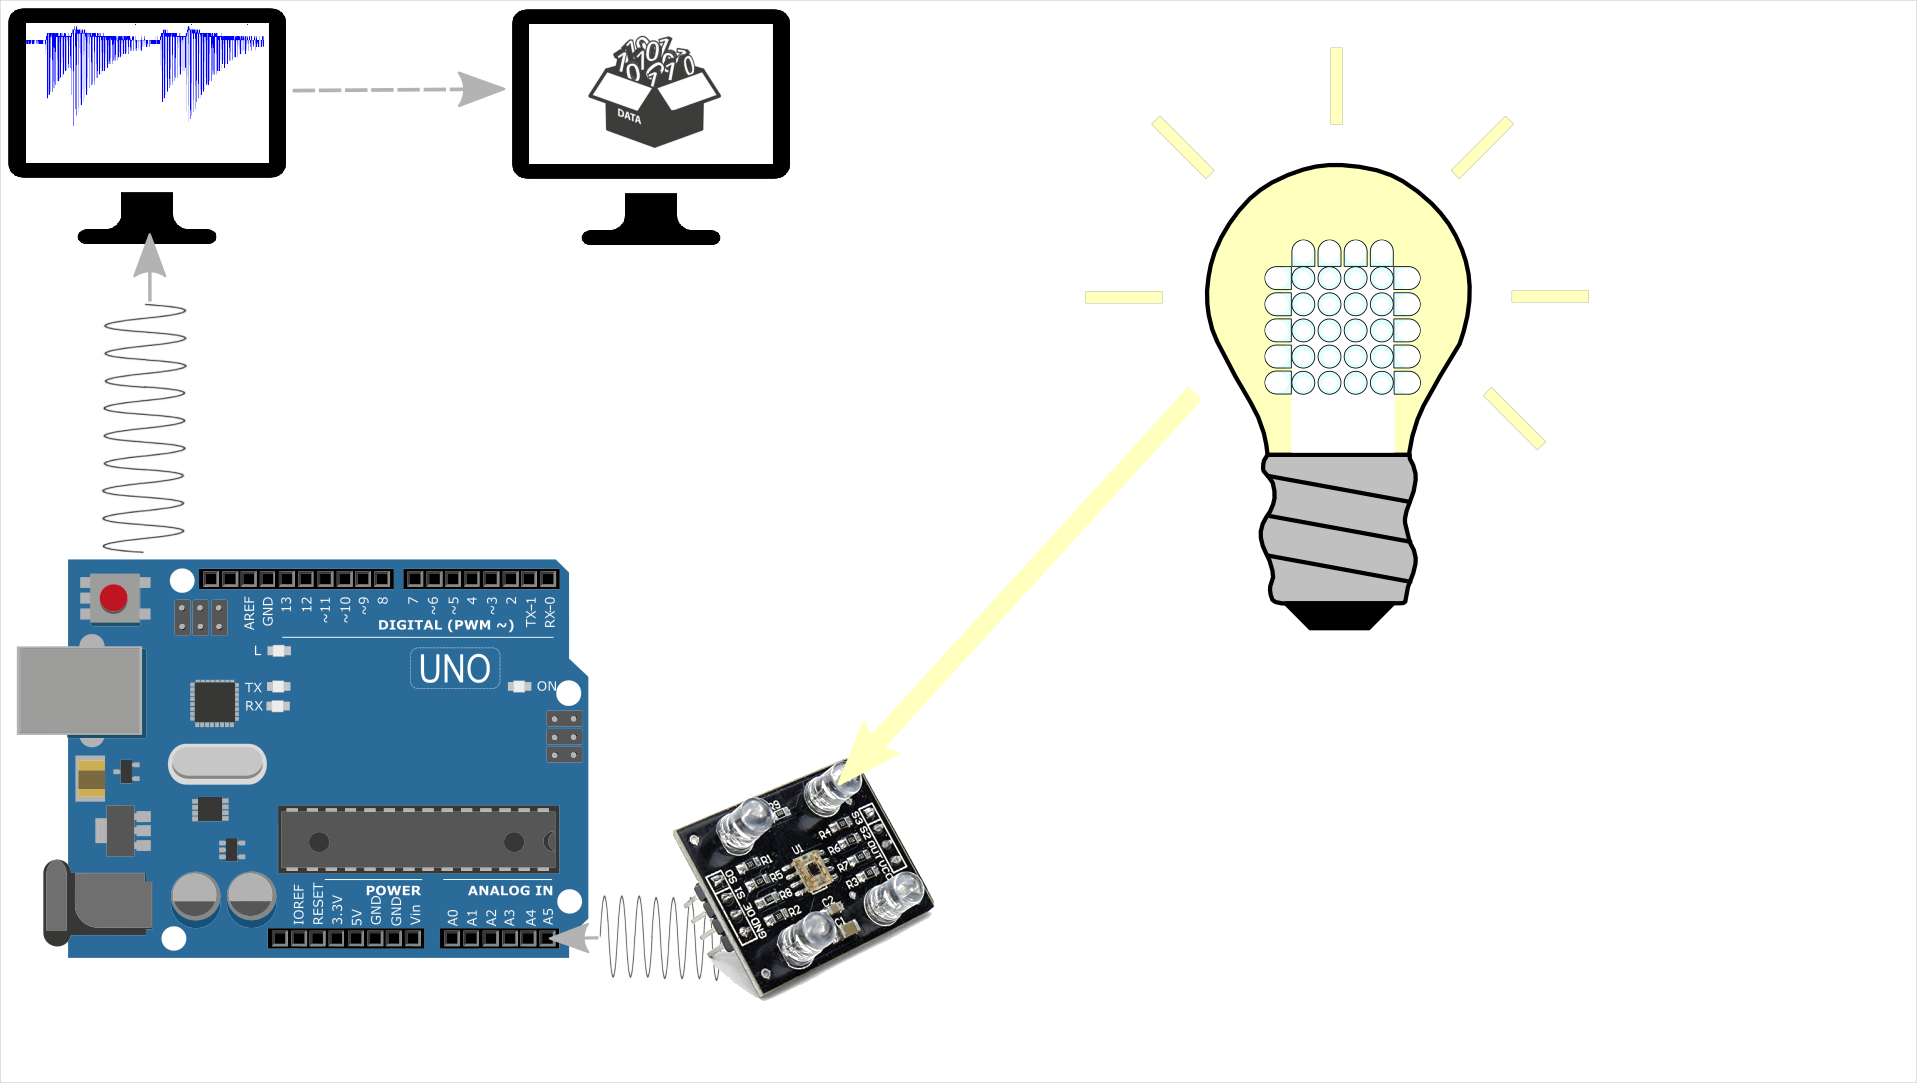
\includegraphics{img/Decoding_5.png}
    }
\end{frame}

\subsubsection{Why this Paper is Important for this Topic}%
\label{sub:why_this_paper_is_important_for_this_topic}
% TODO
% Because it's the only one covering this topic, quite simply^^
\begin{frame}{Why this Paper is Important for our Topic}
    \begin{block}{The One and Only}
        \begin{itemize}
            \item Cluster IoT attacks in presented fashion
            \item Functionality extension attack
            \item Covert Channel on IoT light bulb
        \end{itemize}
    \end{block}
\end{frame}

\begin{frame}{Open Questions regarding our Project} % TODO: please check this slide and change if sth is wrong or add what is missing since I cannot find much information on led versions and according changes...
    \begin{block}{LimitlessLED}
        \begin{itemize}
            \item Faults in API % TODO
            \begin{itemize}
                \item BUT have new API version now
            \end{itemize}
        \end{itemize}
    \end{block}
    
    \begin{block}{Philips Lux}
        \begin{itemize}
            \item Faults in flickering frequence  % TODO
            \begin{itemize}
                \item BUT have new verion of light bulb now
            \end{itemize}
        \end{itemize}
    \end{block}
\end{frame}


%% to show a last slide similar to the title slide: information for the last page
\title{Questions?}
\subtitle{}
\section{Questions}


%% appendix of 'extra' slides
\appendix
\subsection{Epilepsy Triggering Attack}%
\label{sub:epilepsy_triggering_attack}
% TODO Either we only mention it, or we expand it into a full .5 minutes slide.
% Depends on whether we need to fill time I guess.

\begin{frame}[allowframebreaks]{Bibliography}
	\bibliographystyle{alpha}
	\bibliography{../papers/literature.bib}
\end{frame}

\end{document}

% vim: spell ts=2 sw=2
